%%%%%%%%%%%%%%%%%%%%%%%%%%%%%%%%%%%%%%%%%
% Beamer Presentation
% LaTeX Template
% Version 1.0 (10/11/12)
%
% This template has been downloaded from:
% http://www.LaTeXTemplates.com
%
% License:
% CC BY-NC-SA 3.0 (http://creativecommons.org/licenses/by-nc-sa/3.0/)
%
%%%%%%%%%%%%%%%%%%%%%%%%%%%%%%%%%%%%%%%%%

%----------------------------------------------------------------------------------------
%	PACKAGES AND THEMES
%----------------------------------------------------------------------------------------

\documentclass{beamer}

\mode<presentation> {

% The Beamer class comes with a number of default slide themes
% which change the colors and layouts of slides. Below this is a list
% of all the themes, uncomment each in turn to see what they look like.

%\usetheme{default}
%\usetheme{AnnArbor}
%\usetheme{Antibes}
%\usetheme{Bergen}
%\usetheme{Berkeley}
%\usetheme{Berlin}
%\usetheme{Boadilla}
%\usetheme{CambridgeUS}
%\usetheme{Copenhagen}
%\usetheme{Darmstadt}
%\usetheme{Dresden}
%\usetheme{Frankfurt}
%\usetheme{Goettingen}
%\usetheme{Hannover}
%\usetheme{Ilmenau}
%\usetheme{JuanLesPins}
%\usetheme{Luebeck}
\usetheme{Madrid}
%\usetheme{Malmoe}
%\usetheme{Marburg}
%\usetheme{Montpellier}
%\usetheme{PaloAlto}
%\usetheme{Pittsburgh}
%\usetheme{Rochester}
%\usetheme{Singapore}
%\usetheme{Szeged}
%\usetheme{Warsaw}

% As well as themes, the Beamer class has a number of color themes
% for any slide theme. Uncomment each of these in turn to see how it
% changes the colors of your current slide theme.

%\usecolortheme{albatross}
%\usecolortheme{beaver}
%\usecolortheme{beetle}
%\usecolortheme{crane}
%\usecolortheme{dolphin}
%\usecolortheme{dove}
%\usecolortheme{fly}
%\usecolortheme{lily}
%\usecolortheme{orchid}
%\usecolortheme{rose}
%\usecolortheme{seagull}
%\usecolortheme{seahorse}
%\usecolortheme{whale}
%\usecolortheme{wolverine}

%\setbeamertemplate{footline} % To remove the footer line in all slides uncomment this line
%\setbeamertemplate{footline}[page number] % To replace the footer line in all slides with a simple slide count uncomment this line

\setbeamertemplate{navigation symbols}{} % To remove the navigation symbols from the bottom of all slides uncomment this line
}

\usepackage{graphicx} % Allows including images
\usepackage{booktabs} % Allows the use of \toprule, \midrule and \bottomrule in tables
\usepackage[utf8]{inputenc} % Umlaut

%----------------------------------------------------------------------------------------
%	TITLE PAGE
%----------------------------------------------------------------------------------------

\title[Parallel Fringe Search]{Parallel Fringe Search} % The short title appears at the bottom of every slide, the full title is only on the title page

\author{Lukas Mosimann \& Christian Zeman} % Your name
\institute[ETH] % Your institution as it will appear on the bottom of every slide, may be shorthand to save space
{
ETH Zürich \\ % Your institution for the title page
\medskip
\textit{Design of Parallel and High-Performance Computing} % Your email address
}
\date{\today} % Date, can be changed to a custom date

\begin{document}

\begin{frame}
\titlepage % Print the title page as the first slide
\end{frame}

\begin{frame}
\frametitle{Overview} % Table of contents slide, comment this block out to remove it
\tableofcontents % Throughout your presentation, if you choose to use \section{} and \subsection{} commands, these will automatically be printed on this slide as an overview of your presentation
\end{frame}

%----------------------------------------------------------------------------------------
%	PRESENTATION SLIDES
%----------------------------------------------------------------------------------------

%------------------------------------------------
\section{Fringe Search} % Sections can be created in order to organize your presentation into discrete blocks, all sections and subsections are automatically printed in the table of contents as an overview of the talk
%------------------------------------------------

\begin{frame}
\frametitle{Fringe Search}
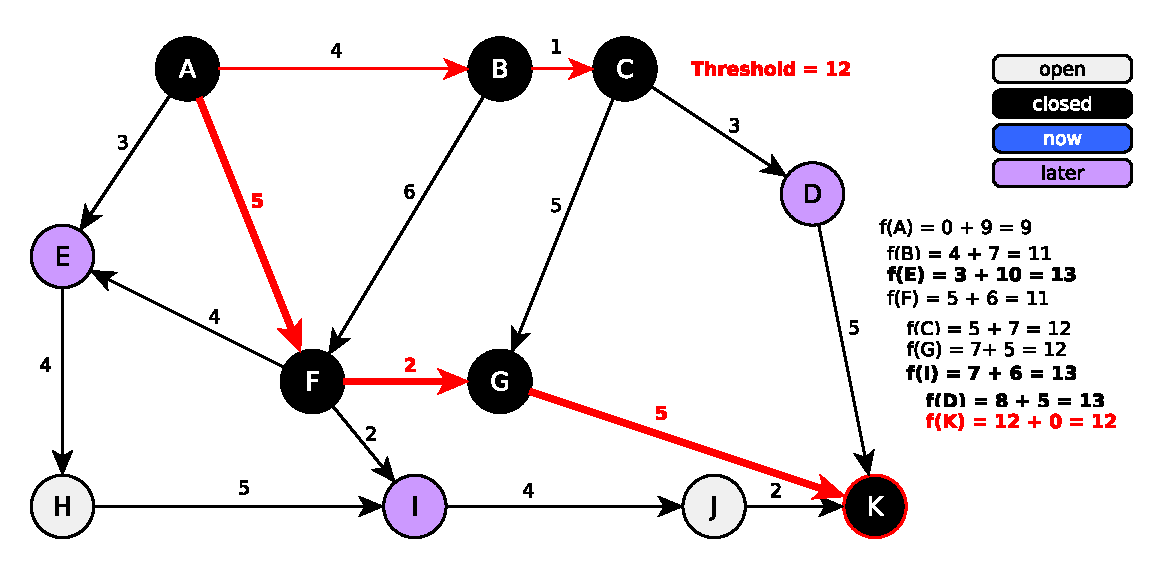
\includegraphics[height=165pt]{fringe7.pdf}
\end{frame}

%------------------------------------------------
\section{What we have done}
%------------------------------------------------

\begin{frame}
\frametitle{What we have done}
\begin{itemize}
\item Serial implementation of fringe search (much faster than Boost A*)
\item Parallel implementation with Open MP
	\begin{itemize}
	\item 2 different locking concepts
	\item Locks implemented using inline assembly (faster than Open MP locks)
	\end{itemize}
\item Benchmarking
	\begin{itemize}
	\item Strong scaling
	\item Weak scaling
	\item Path quality
	\end{itemize}
\end{itemize}
\end{frame}

%------------------------------------------------
\section{Locking concepts}
%------------------------------------------------

\begin{frame}
\frametitle{Locking concept: Deadlock prevention}
\begin{center}
	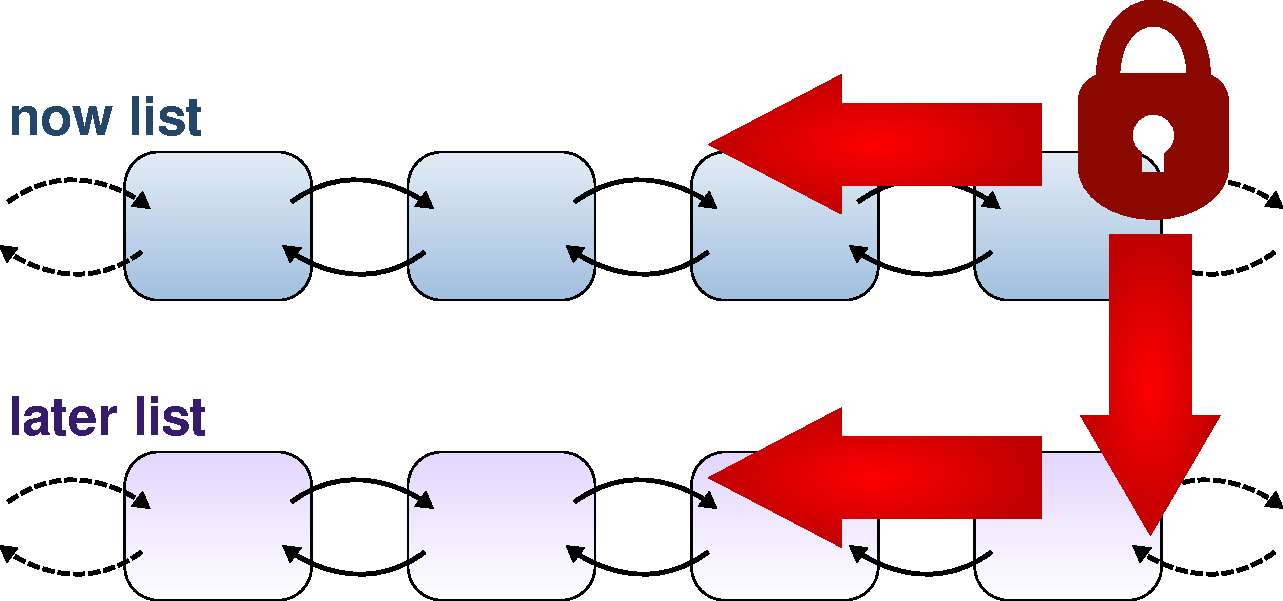
\includegraphics[height=140pt]{locking.pdf}
\end{center}
\end{frame}

\begin{frame}
\frametitle{Locking concept: Insert node}
\begin{center}
	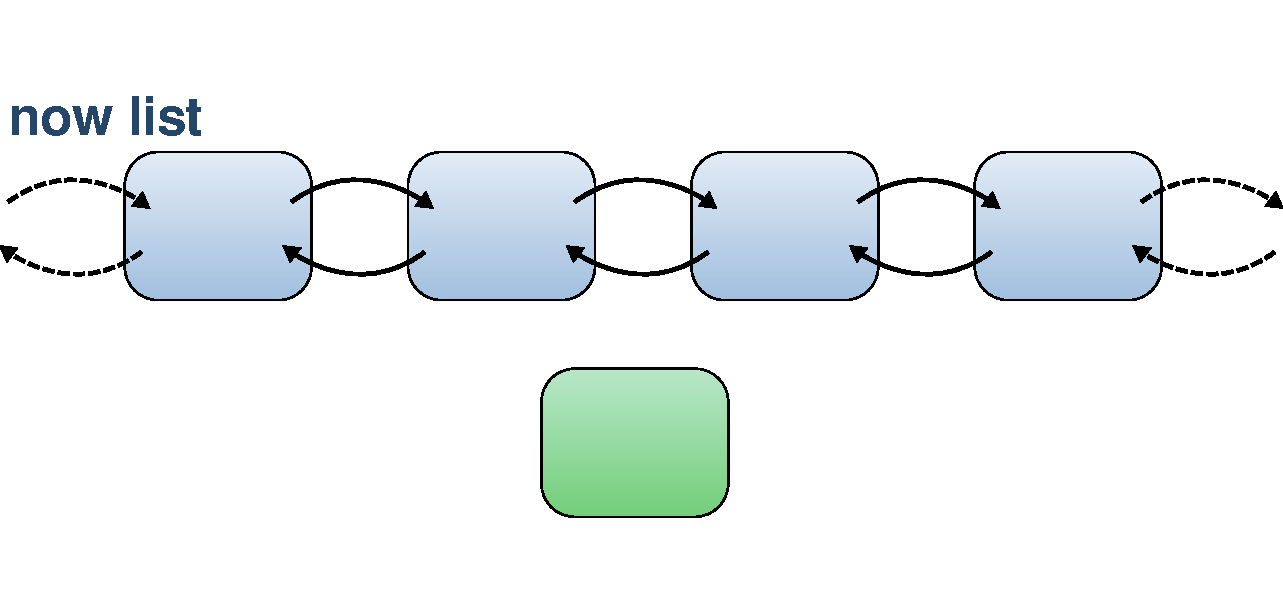
\includegraphics[height=140pt]{insert1.pdf}
\end{center}
\end{frame}

\begin{frame}
\frametitle{Locking concept: Insert node}
\begin{center}
	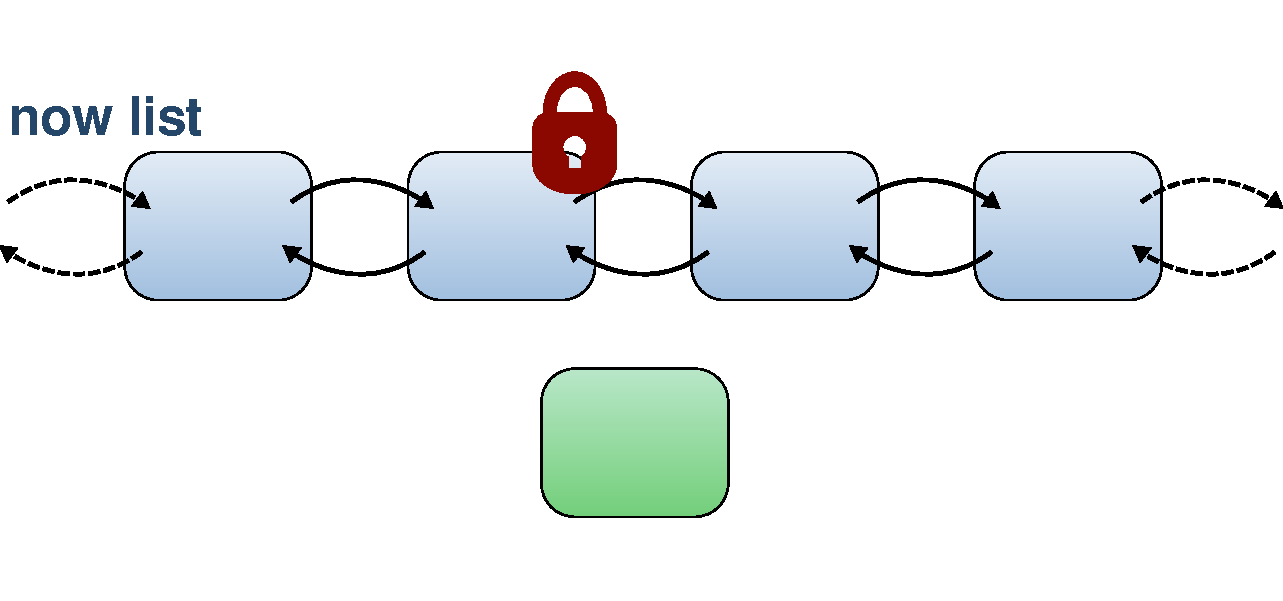
\includegraphics[height=140pt]{insert2.pdf}
\end{center}
\end{frame}

\begin{frame}
\frametitle{Locking concept: Insert node}
\begin{center}
	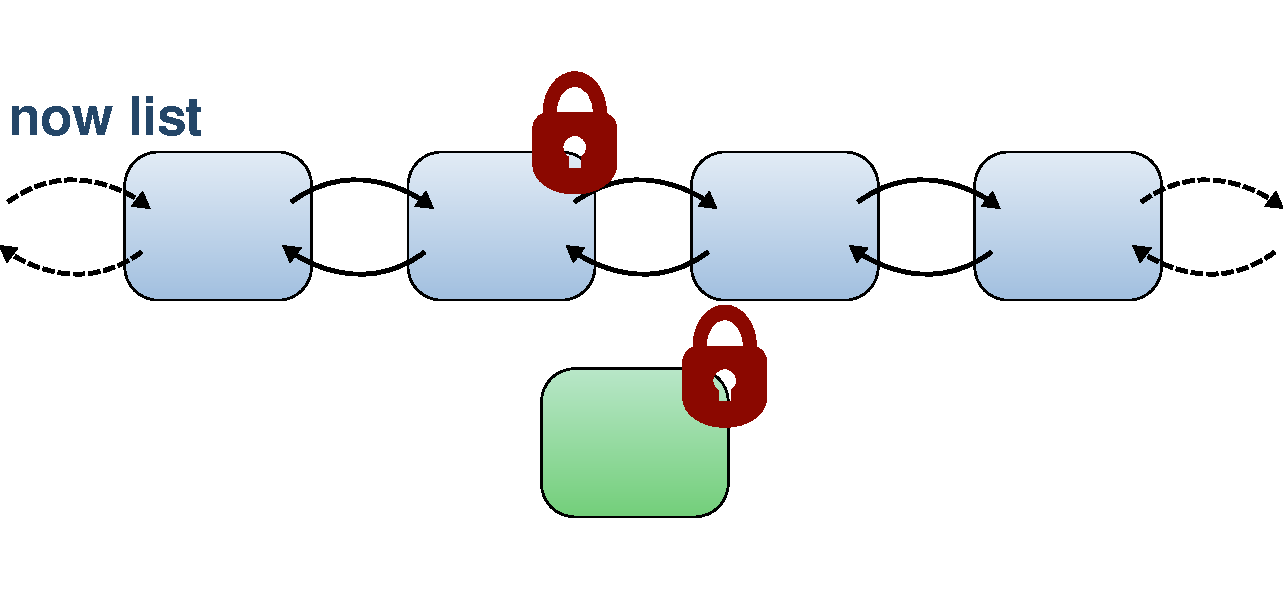
\includegraphics[height=140pt]{insert2b.pdf}
\end{center}
\end{frame}

\begin{frame}
\frametitle{Locking concept: Insert node}
\begin{center}
	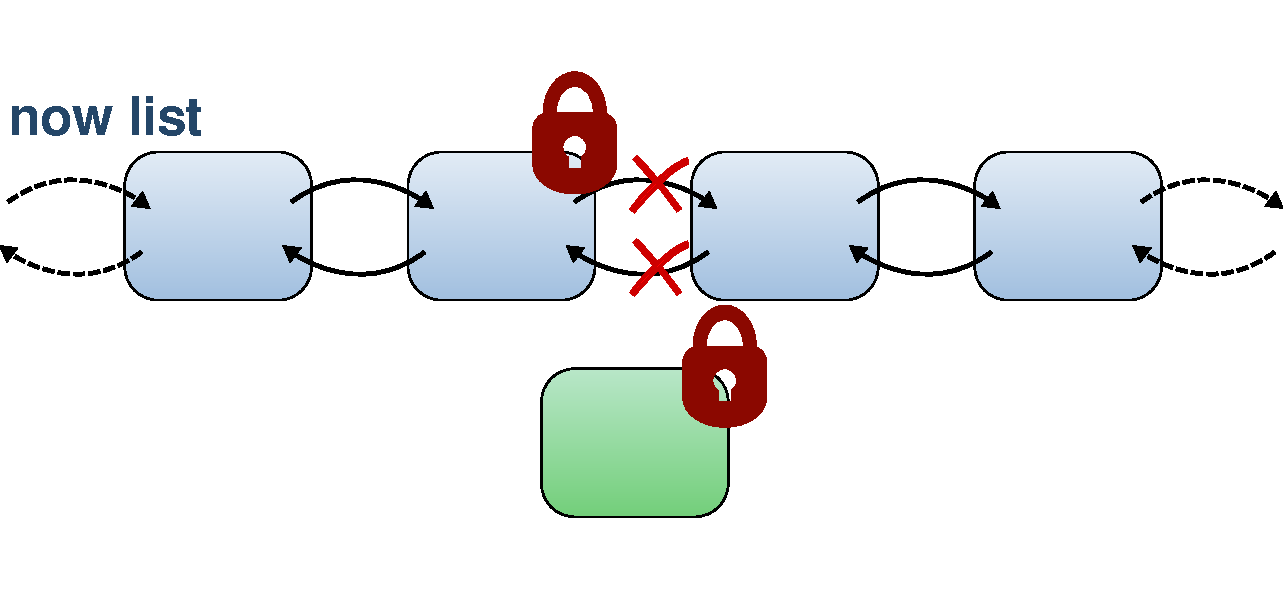
\includegraphics[height=140pt]{insert3.pdf}
\end{center}
\end{frame}

\begin{frame}
\frametitle{Locking concept: Insert node}
\begin{center}
	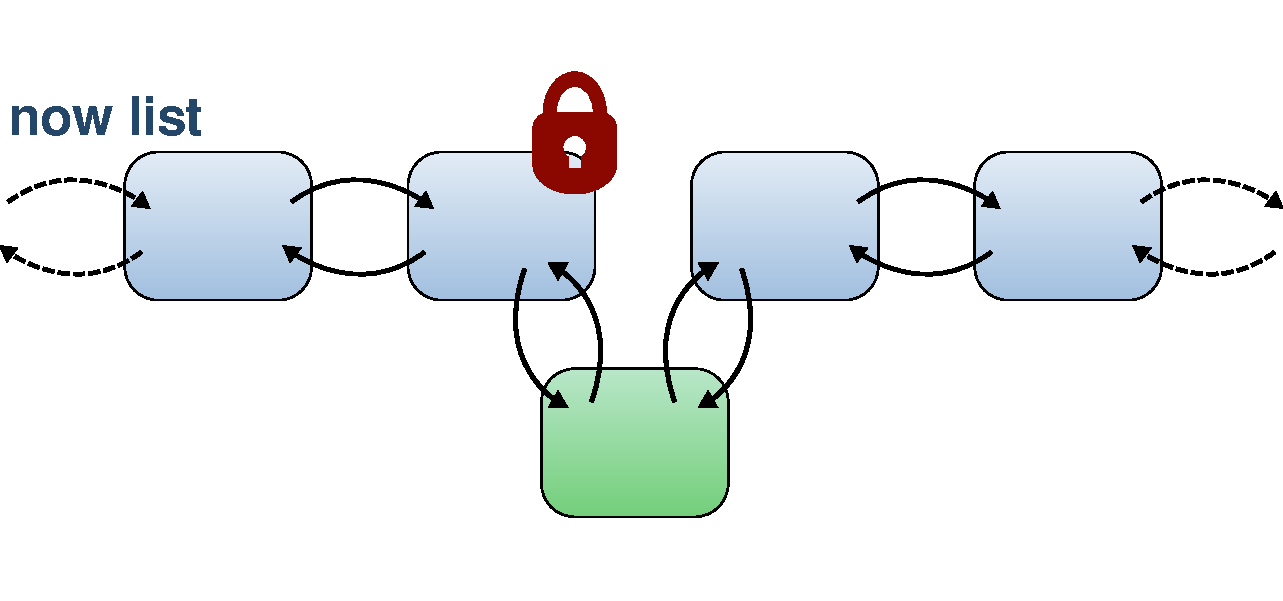
\includegraphics[height=140pt]{insert4.pdf}
\end{center}
\end{frame}

\begin{frame}
\frametitle{Locking concept: Insert node}
\begin{center}
	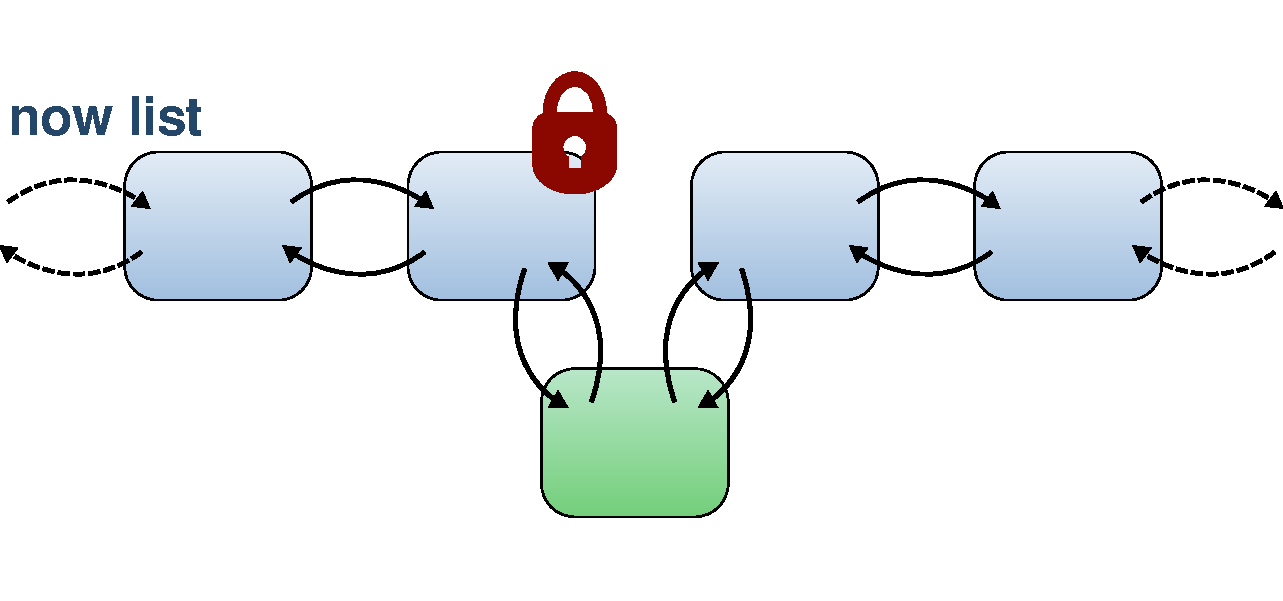
\includegraphics[height=140pt]{insert5.pdf}
\end{center}
\end{frame}

\begin{frame}
\frametitle{Locking concept: Insert node}
\begin{center}
	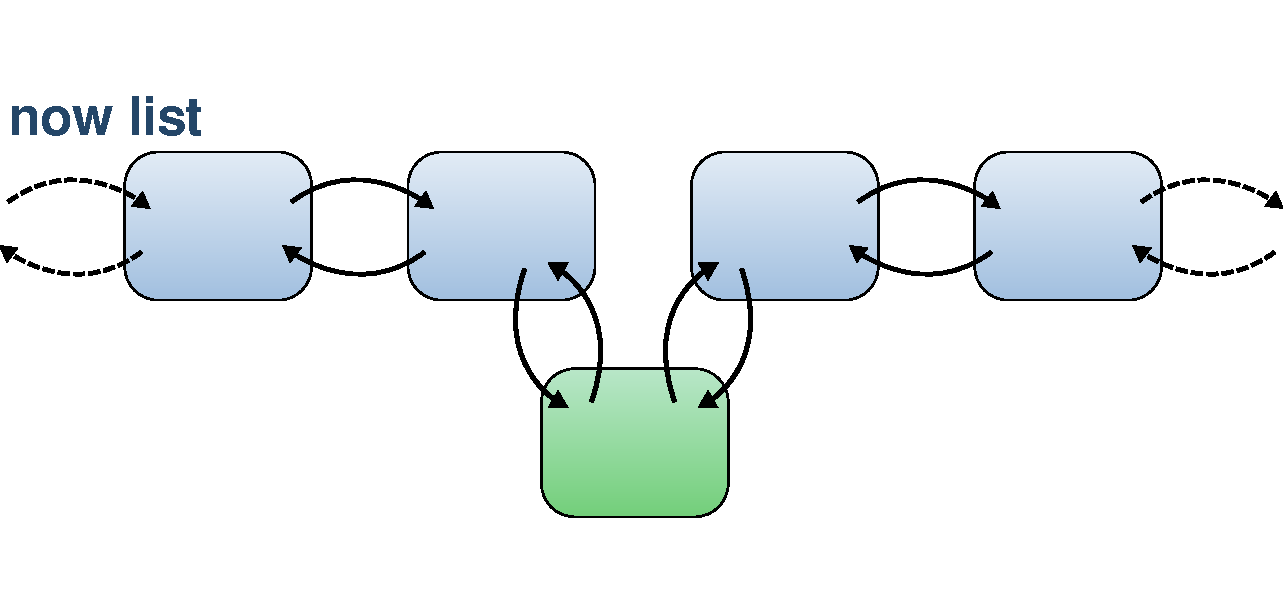
\includegraphics[height=140pt]{insert6.pdf}
\end{center}
\end{frame}

%------------------------------------------------

\begin{frame}
\frametitle{Locking concept: Remove node}
\begin{center}
	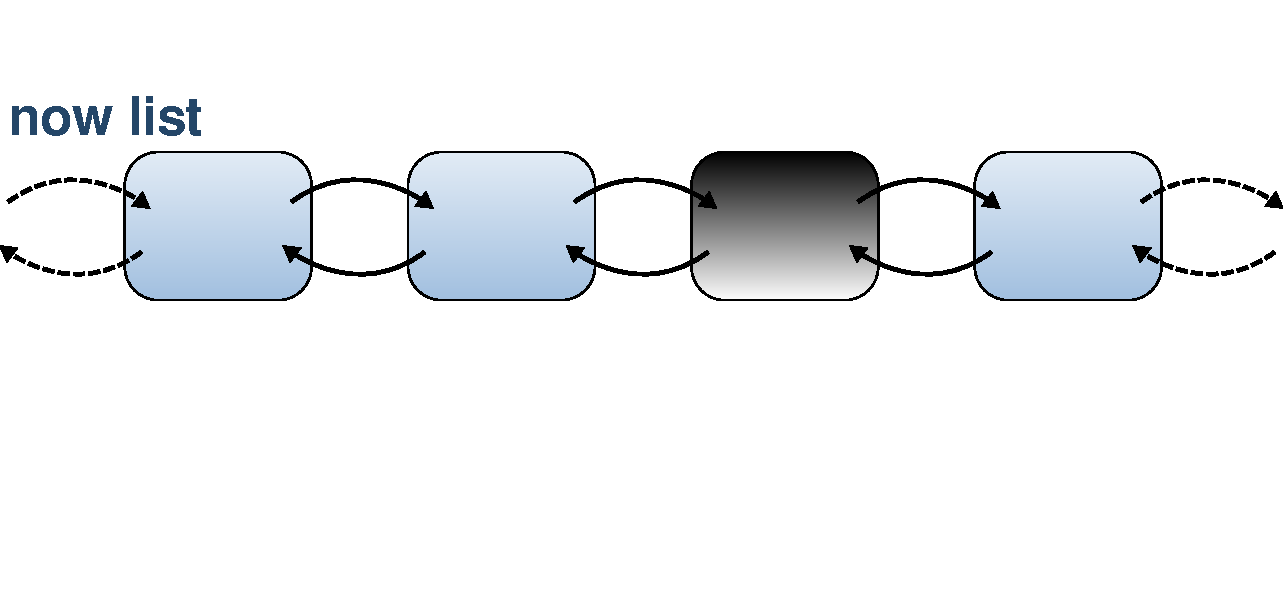
\includegraphics[height=140pt]{remove1.pdf}
\end{center}
\end{frame}

\begin{frame}
\frametitle{Locking concept: Remove node}
\begin{center}
	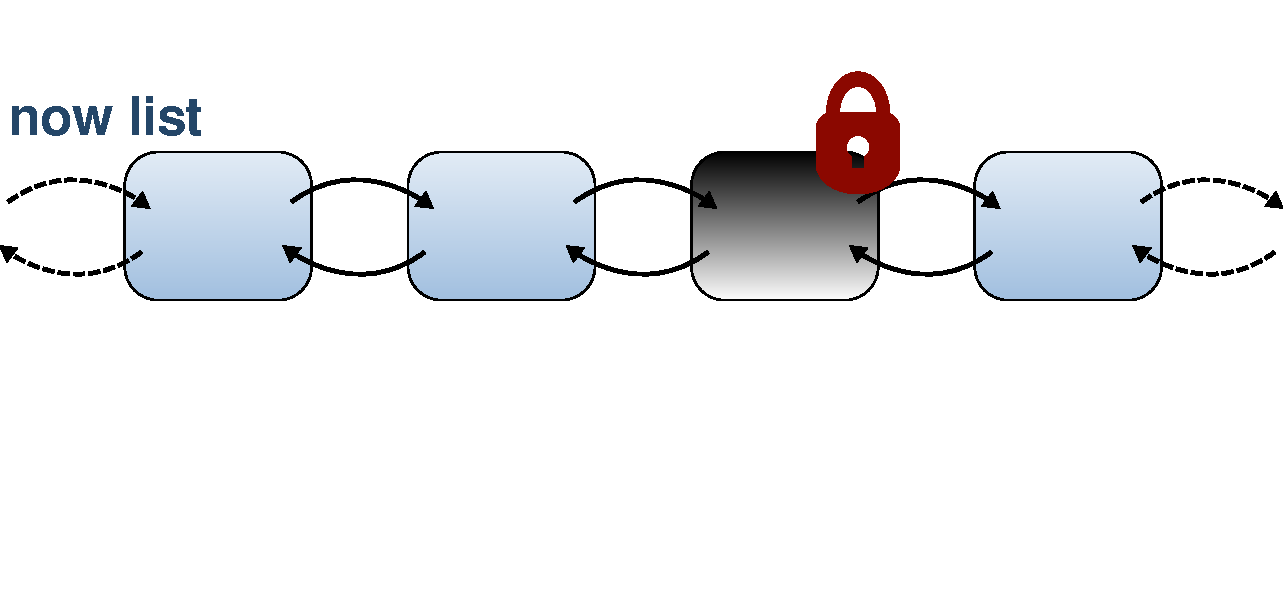
\includegraphics[height=140pt]{remove2.pdf}
\end{center}
\end{frame}

\begin{frame}
\frametitle{Locking concept: Remove node}
\begin{center}
	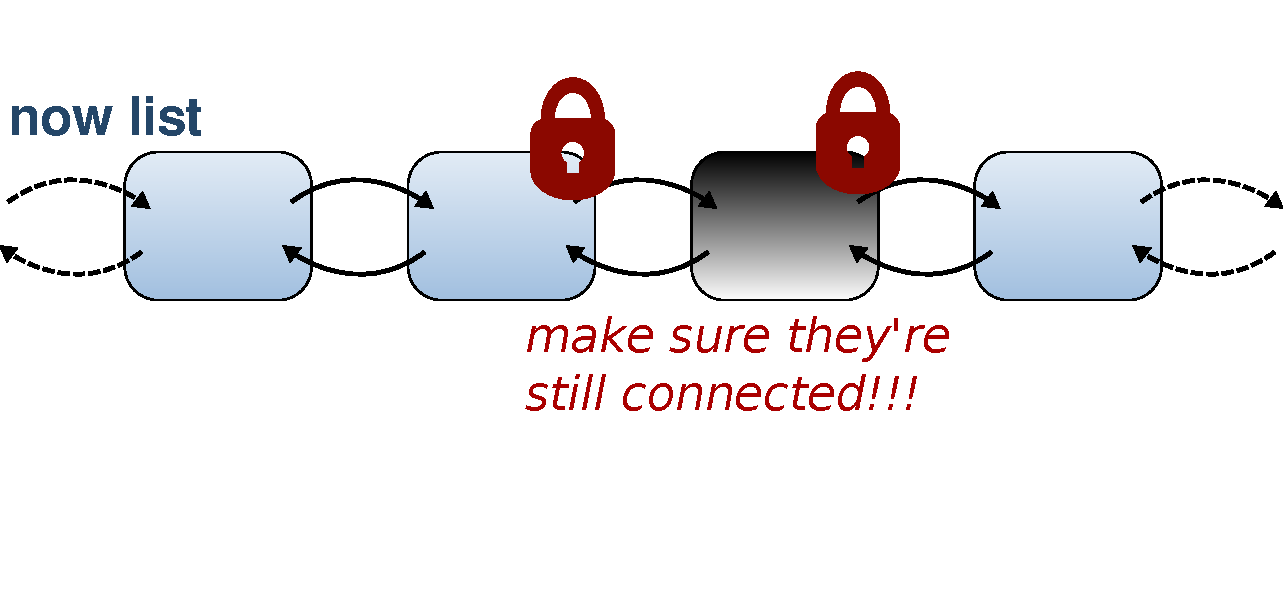
\includegraphics[height=140pt]{remove3.pdf}
\end{center}
\end{frame}

\begin{frame}
\frametitle{Locking concept: Remove node}
\begin{center}
	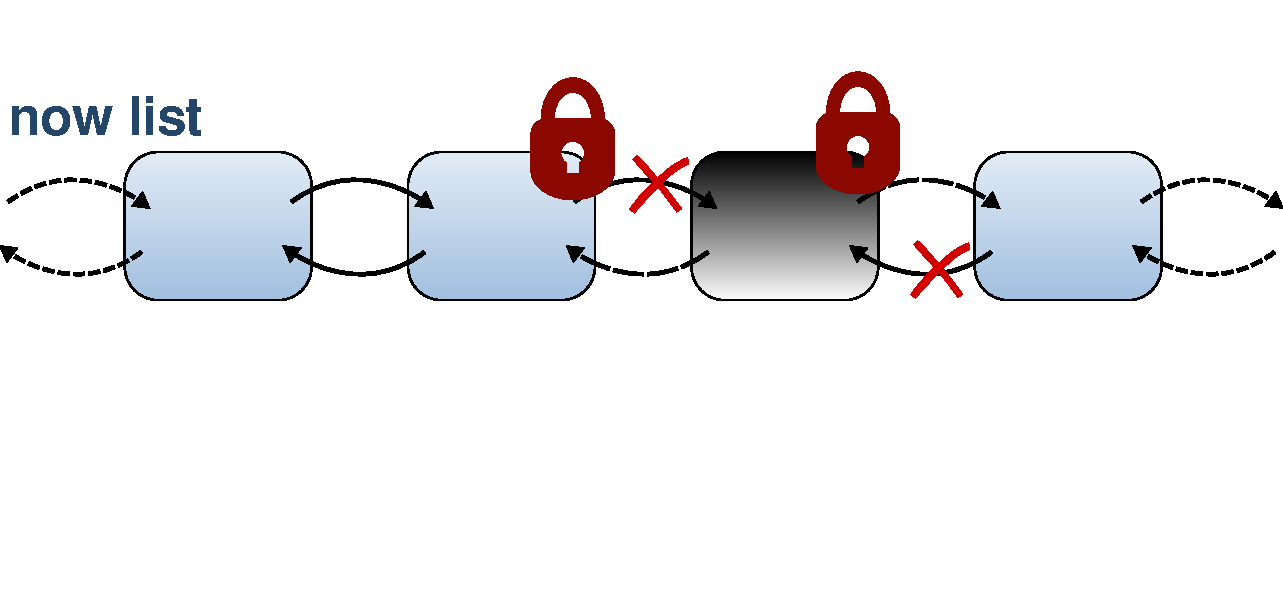
\includegraphics[height=140pt]{remove4.pdf}
\end{center}
\end{frame}

\begin{frame}
\frametitle{Locking concept: Remove node}
\begin{center}
	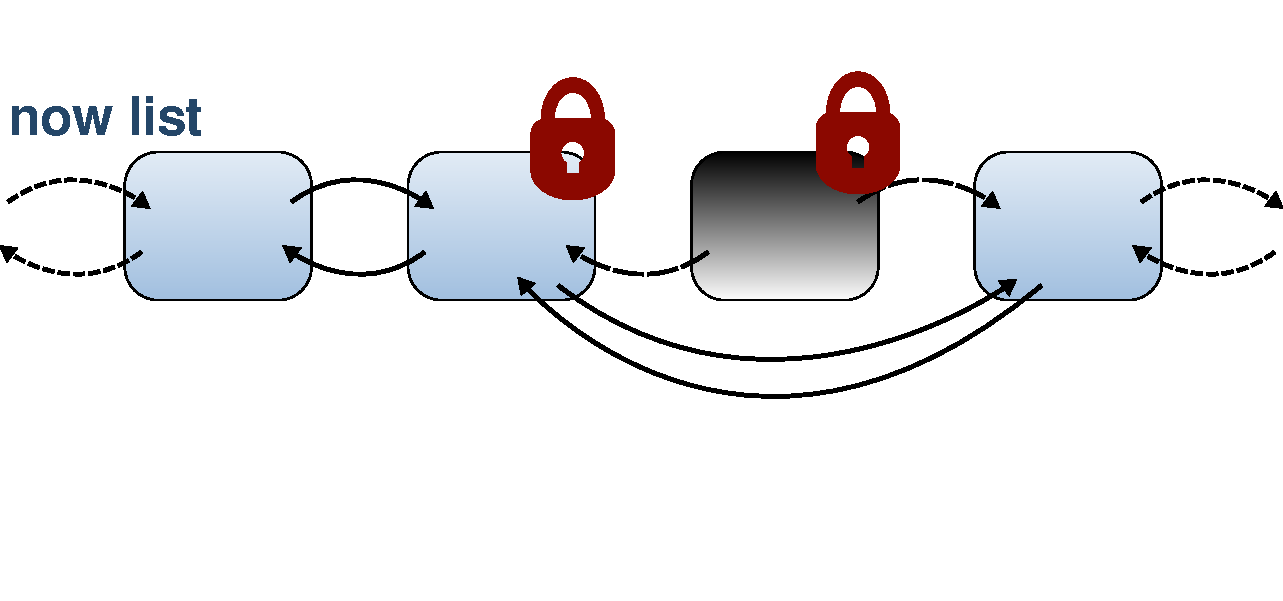
\includegraphics[height=140pt]{remove5.pdf}
\end{center}
\end{frame}

\begin{frame}
\frametitle{Locking concept: Remove node}
\begin{center}
	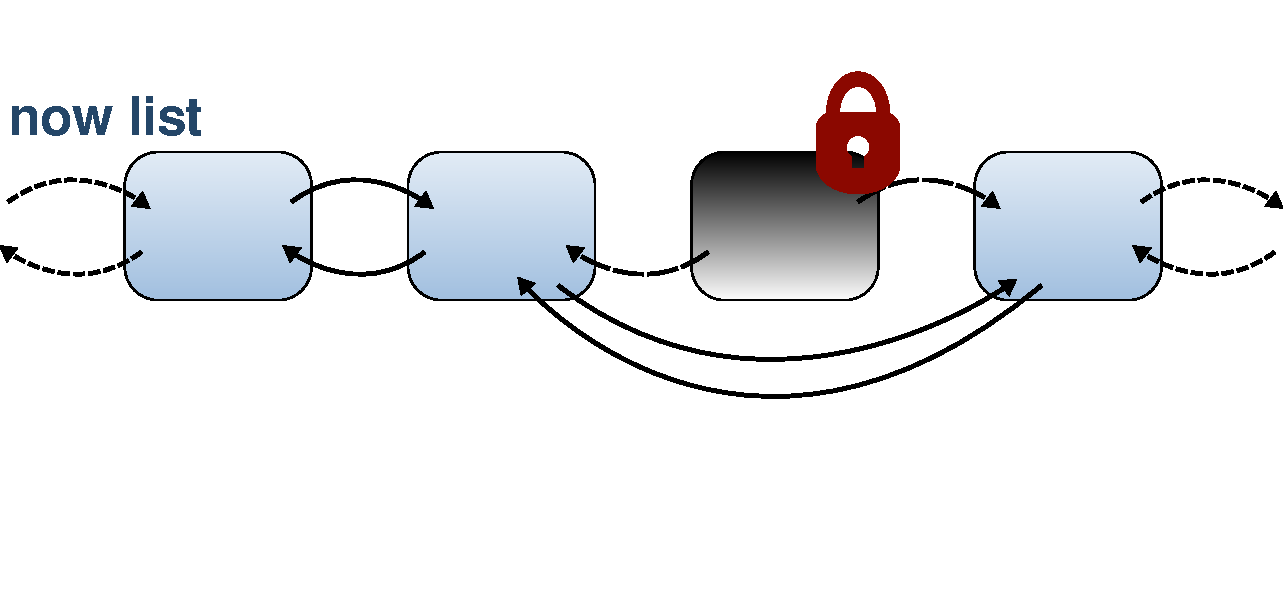
\includegraphics[height=140pt]{remove6.pdf}
\end{center}
\end{frame}

\begin{frame}
\frametitle{Locking concept: Remove node}
\begin{center}
	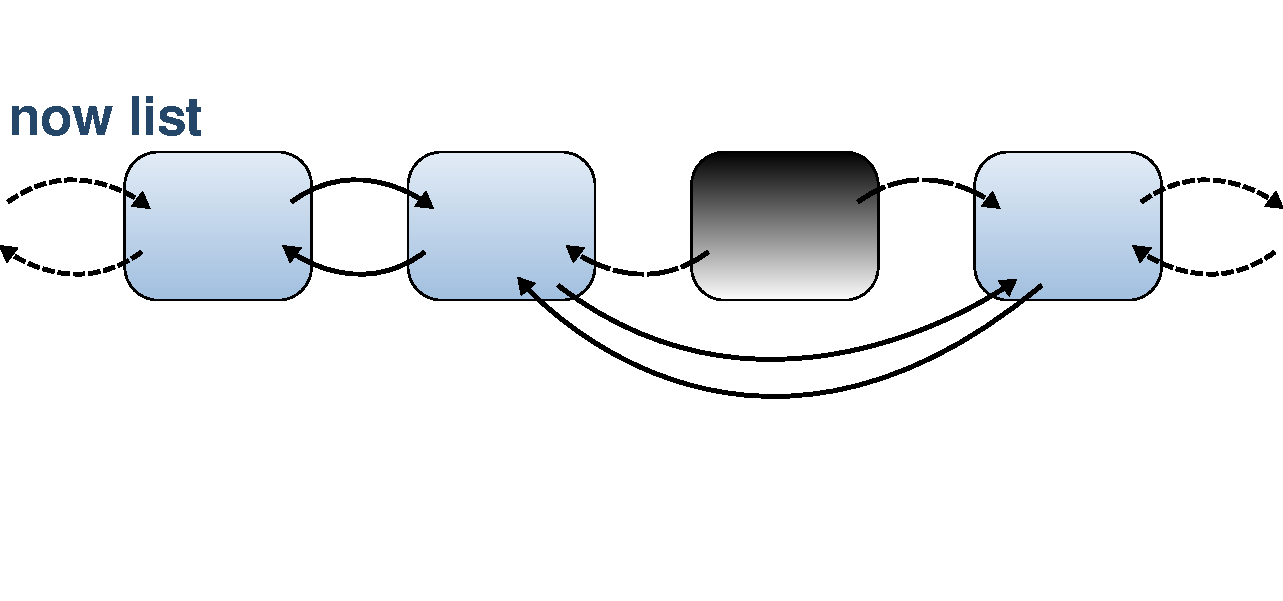
\includegraphics[height=140pt]{remove7.pdf}
\end{center}
\end{frame}

%------------------------------------------------

\begin{frame}
\frametitle{Locking concept: 2 concepts for removing nodes}
Both concepts use optimistic locking for acquiring the locks.\\
\quad\\
\textbf{Normal:}
\begin{itemize}
\item Lock node and predecessor as shown before and remove it right away
\end{itemize}
\quad\\ \quad \\
\textbf{Lazy locking:}
\begin{itemize}
\item Don't lock anything and just mark the node as removed
\item Other threads will clean up and remove it later
\end{itemize}

\end{frame}

%------------------------------------------------
\section{Benchmarks}
%------------------------------------------------

\begin{frame}
\frametitle{Benchmarking}
\textbf{Setup:}\\ \quad\\
Each of the following boxplots was generated from data from \textbf{50 runs} on \textbf{1 node} of kanifushi.inf.ethz.ch.\\
\quad\\
Specifications of kanifushi.inf.ethz.ch:
\begin{itemize}
\item NUMA model with 32 CPUs on 4 nodes
\item 8 CPUs per node
\item Intel(R) Xeon(R) CPU E7- 4830  @ 2.13GHz
\item per CPU: 32KB L1 cache, 256KB L2 cache
\item per node: 24MB L3 cache, 16GB memory
\end{itemize}
\quad\\ \quad\\
The code is written in C++ / Open MP and it has been compiled with g++ v. 4.6.1 using O1 optimization.
\end{frame}

\begin{frame}
\frametitle{Benchmarking}
\begin{columns}[c] % The "c" option specifies centered vertical alignment while the "t" option is used for top vertical alignment
\column{.6\textwidth} % Left column and width
\textbf{Graphs}
\begin{itemize}
\item based on a regular grid with distance 1 and 8 edges per node
\item each node  is moved randomly\\(normal distribution, $\sigma = 0.3$)
\item different obstacles (circle, crosses, etc.)
\vspace{10pt}
\begin{center}
	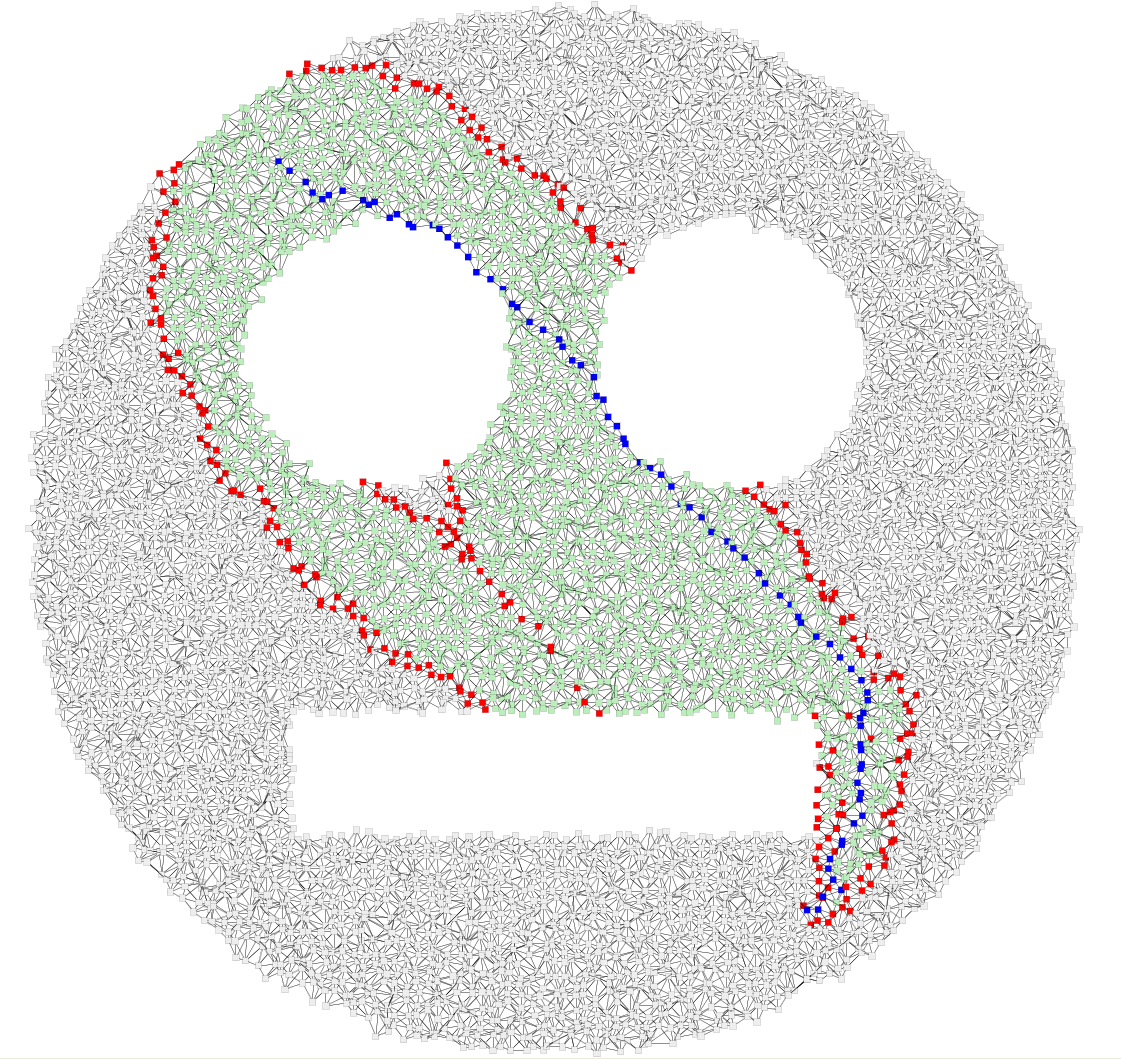
\includegraphics[height=120pt]{smiley.pdf}
\end{center}
\end{itemize}

\column{.4\textwidth} % Right column and width
\begin{center}
	\includegraphics[height=210pt]{two_graphs.pdf}
\end{center}
\end{columns}
\end{frame}

\begin{frame}
\frametitle{Benchmarking}
\begin{columns}[c] % The "c" option specifies centered vertical alignment while the "t" option is used for top vertical alignment
\column{.6\textwidth} % Left column and width
\textbf{Graphs}
\begin{itemize}
\item based on a regular grid with distance 1 and 8 edges per node
\item each node  is moved randomly\\(normal distribution, $\sigma$ = 0.3)
\item different obstacles (circle, crosses, etc.)
\vspace{10pt}
\begin{center}
	\includegraphics[height=120pt]{smiley_zoom1.pdf}
\end{center}
\end{itemize}

\column{.4\textwidth} % Right column and width
\begin{center}
	\includegraphics[height=210pt]{two_graphs.pdf}
\end{center}
\end{columns}
\end{frame}

\begin{frame}
\frametitle{Benchmarking}
\begin{columns}[c] % The "c" option specifies centered vertical alignment while the "t" option is used for top vertical alignment
\column{.6\textwidth} % Left column and width
\textbf{Graphs}
\begin{itemize}
\item based on a regular grid with distance 1 and 8 edges per node
\item each node  is moved randomly\\(normal distribution, $\sigma$ = 0.3)
\item different obstacles (circle, crosses, etc.)
\vspace{10pt}
\begin{center}
	\includegraphics[height=120pt]{zoom.pdf}
\end{center}
\end{itemize}

\column{.4\textwidth} % Right column and width
\begin{center}
	\includegraphics[height=210pt]{two_graphs.pdf}
\end{center}
\end{columns}
\end{frame}


%------------------------------------------------
\subsection{Locks}
\begin{frame}
\frametitle{Benchmarking: Locks}
\begin{center}
	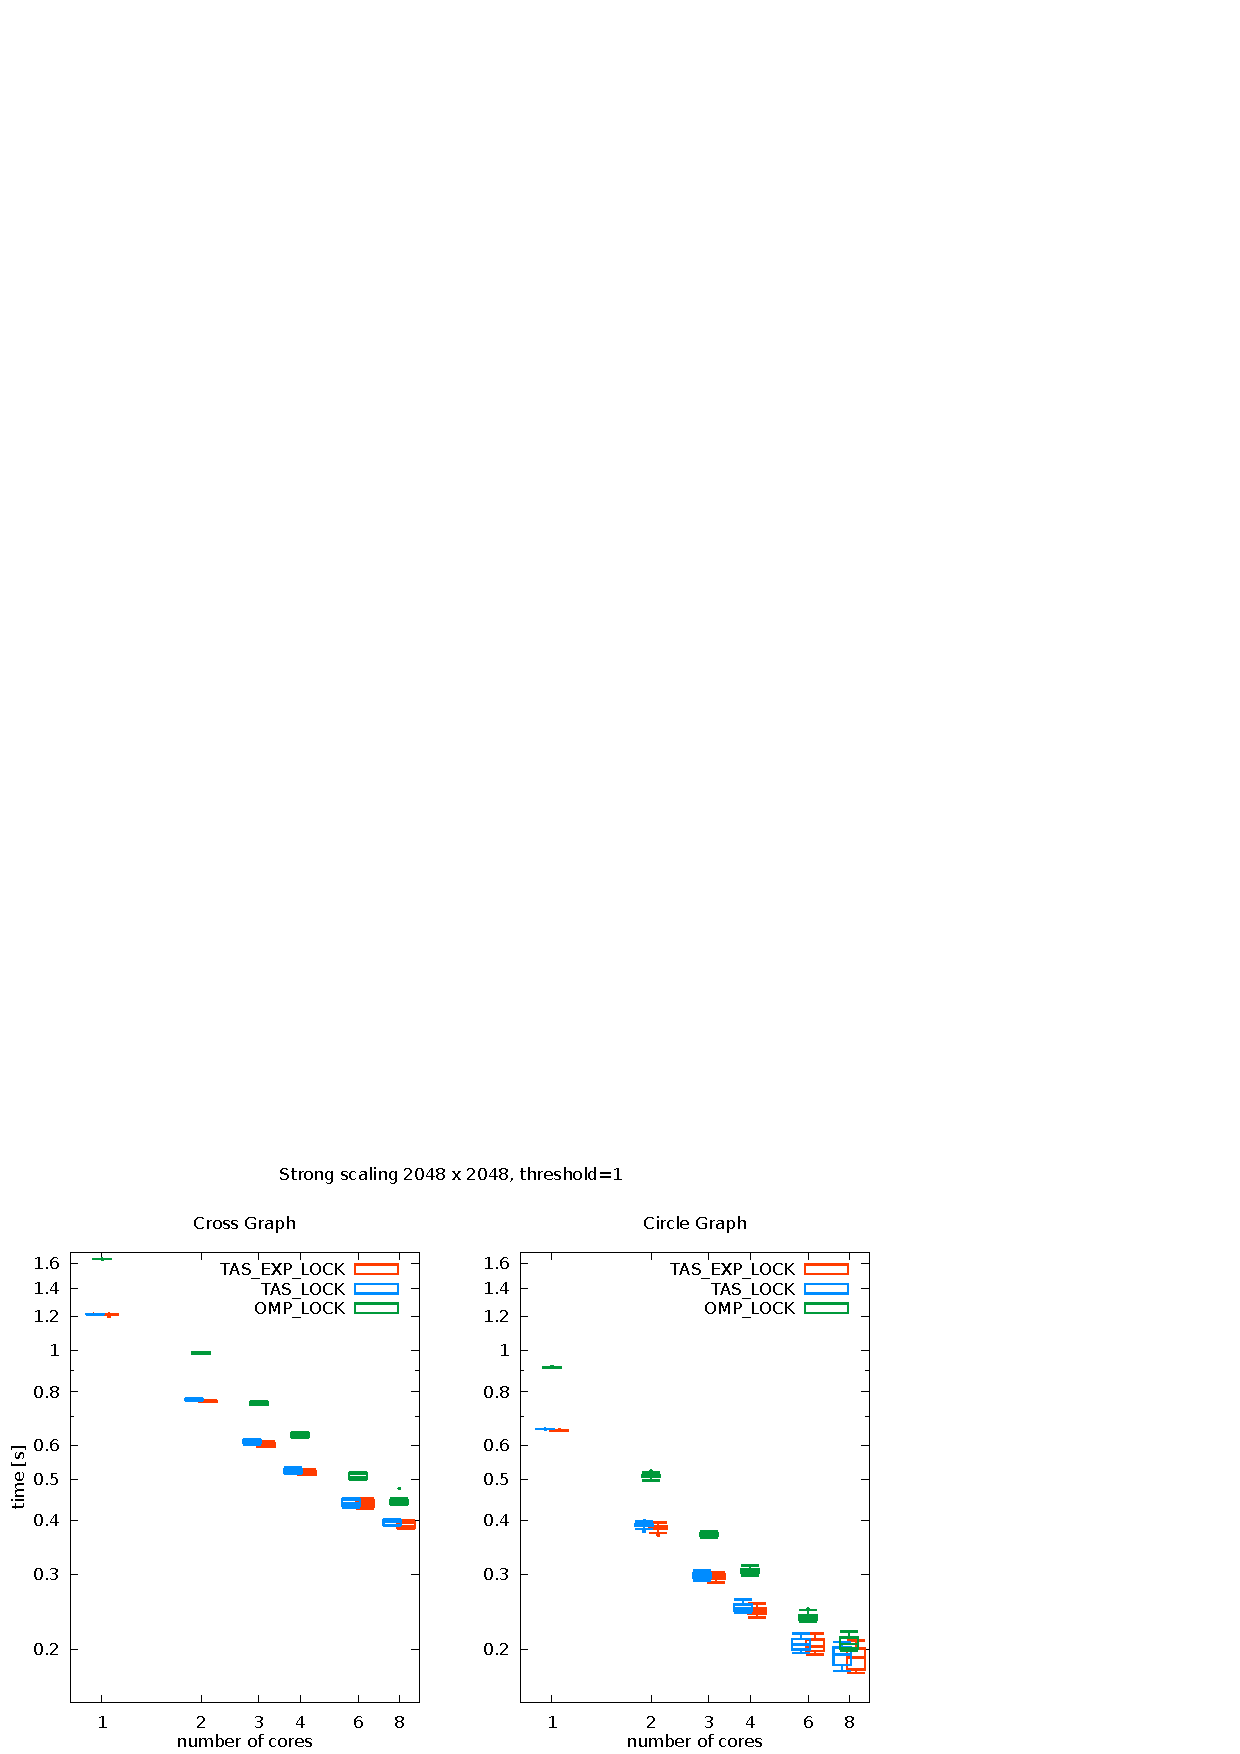
\includegraphics[height=210pt]{lock_benchmark.pdf}
\end{center}
\end{frame}

%------------------------------------------------
\subsection{Strong scaling}
\begin{frame}
\frametitle{Benchmarking: Strong scaling}
\begin{center}
	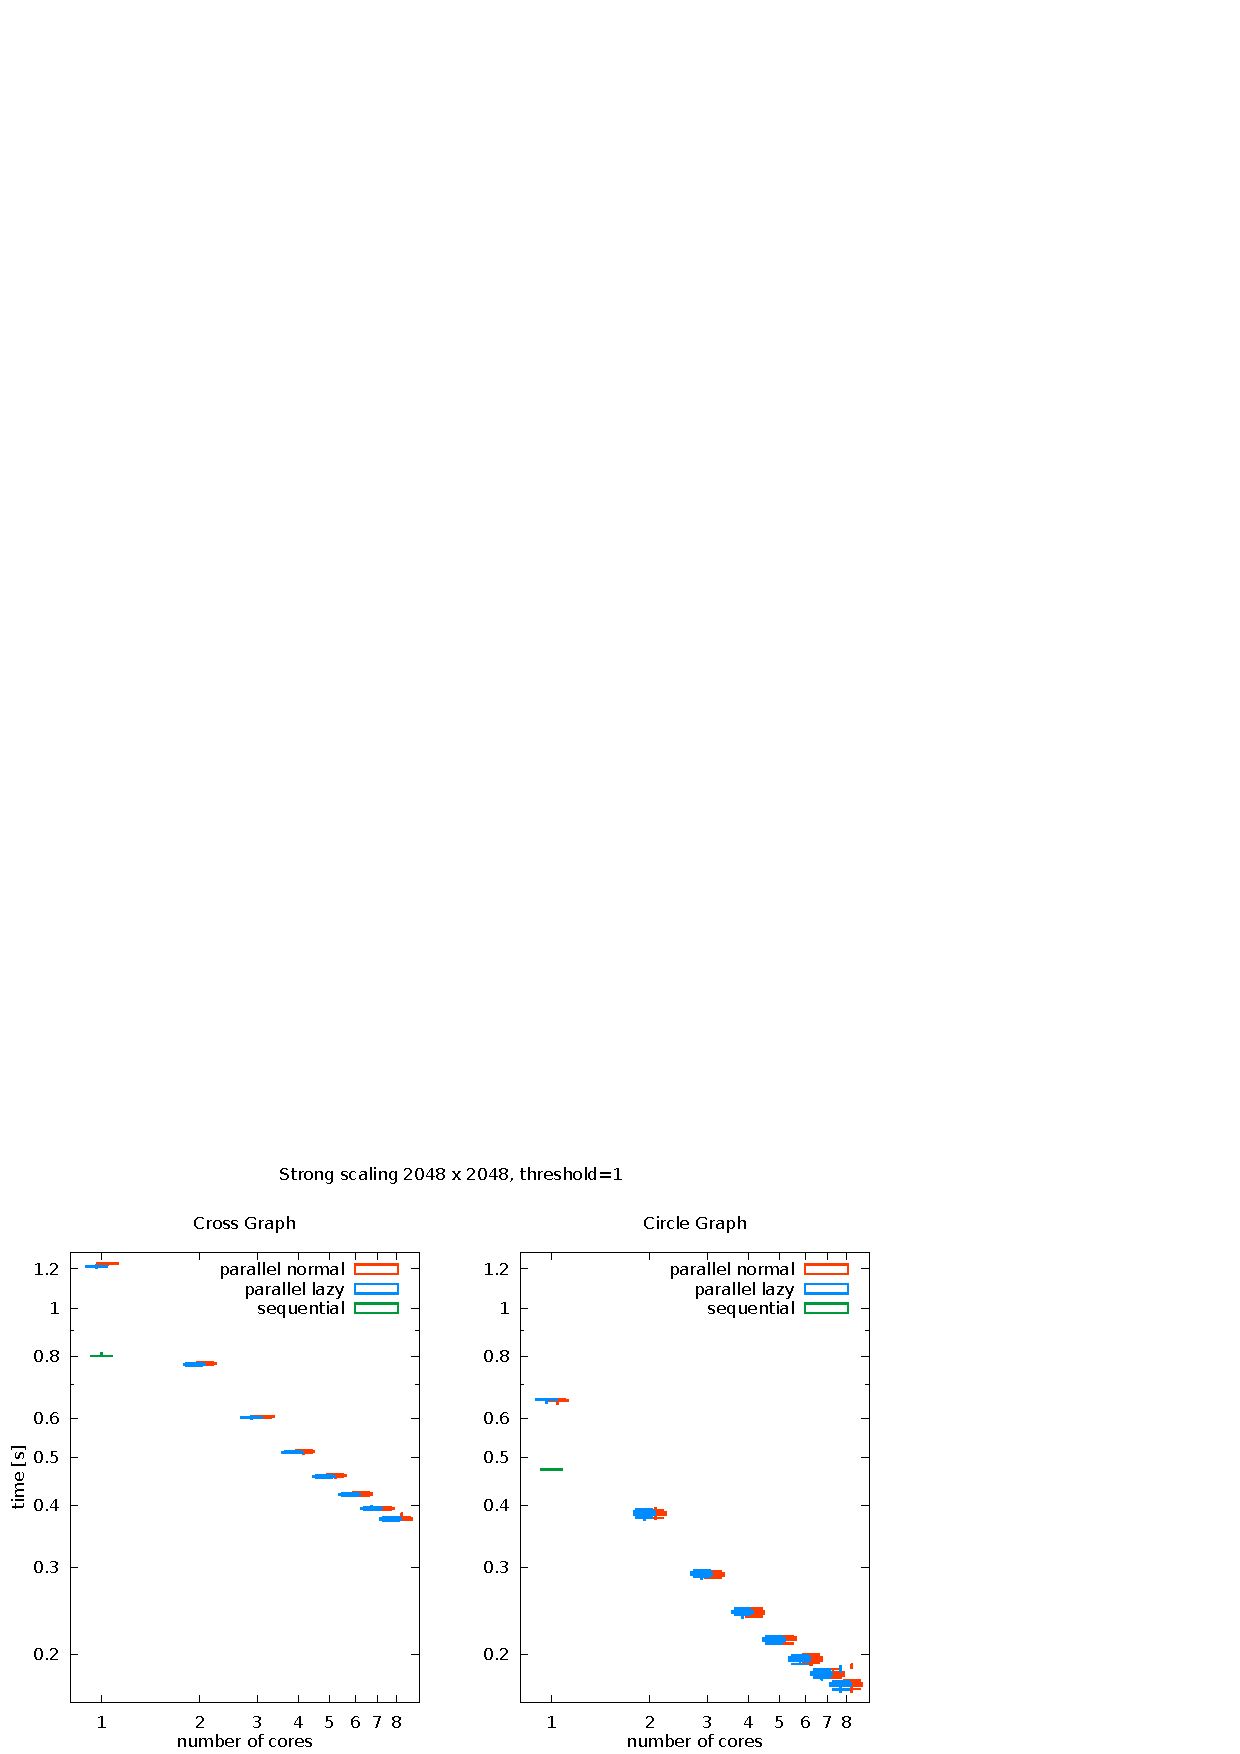
\includegraphics[height=210pt]{strong_scaling.pdf}
\end{center}
\end{frame}

%------------------------------------------------
\subsection{Weak scaling}
\begin{frame}
\frametitle{Benchmarking: Sequential scaling}
\begin{center}
	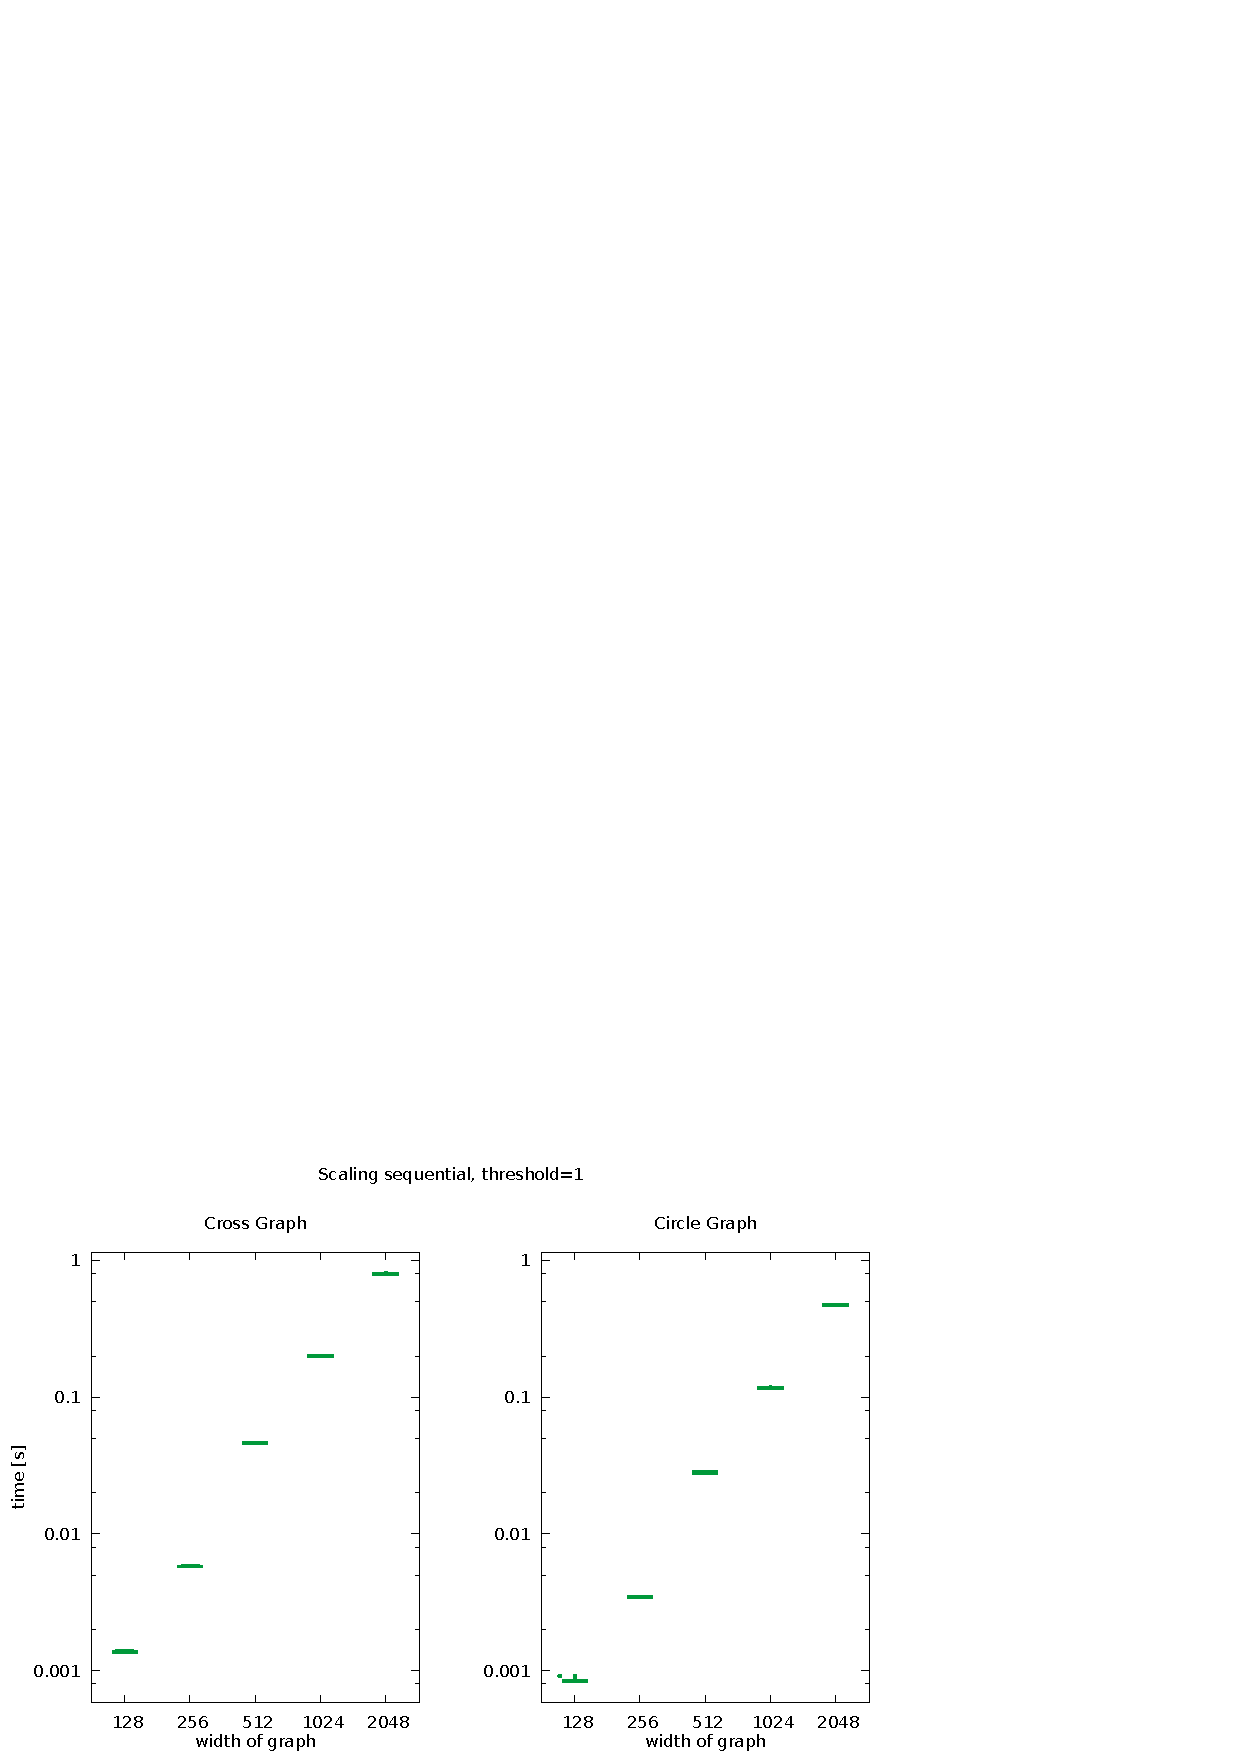
\includegraphics[height=210pt]{seq_scaling.pdf}
\end{center}
\end{frame}

\begin{frame}
\frametitle{Benchmarking: Weak scaling}
\begin{center}
	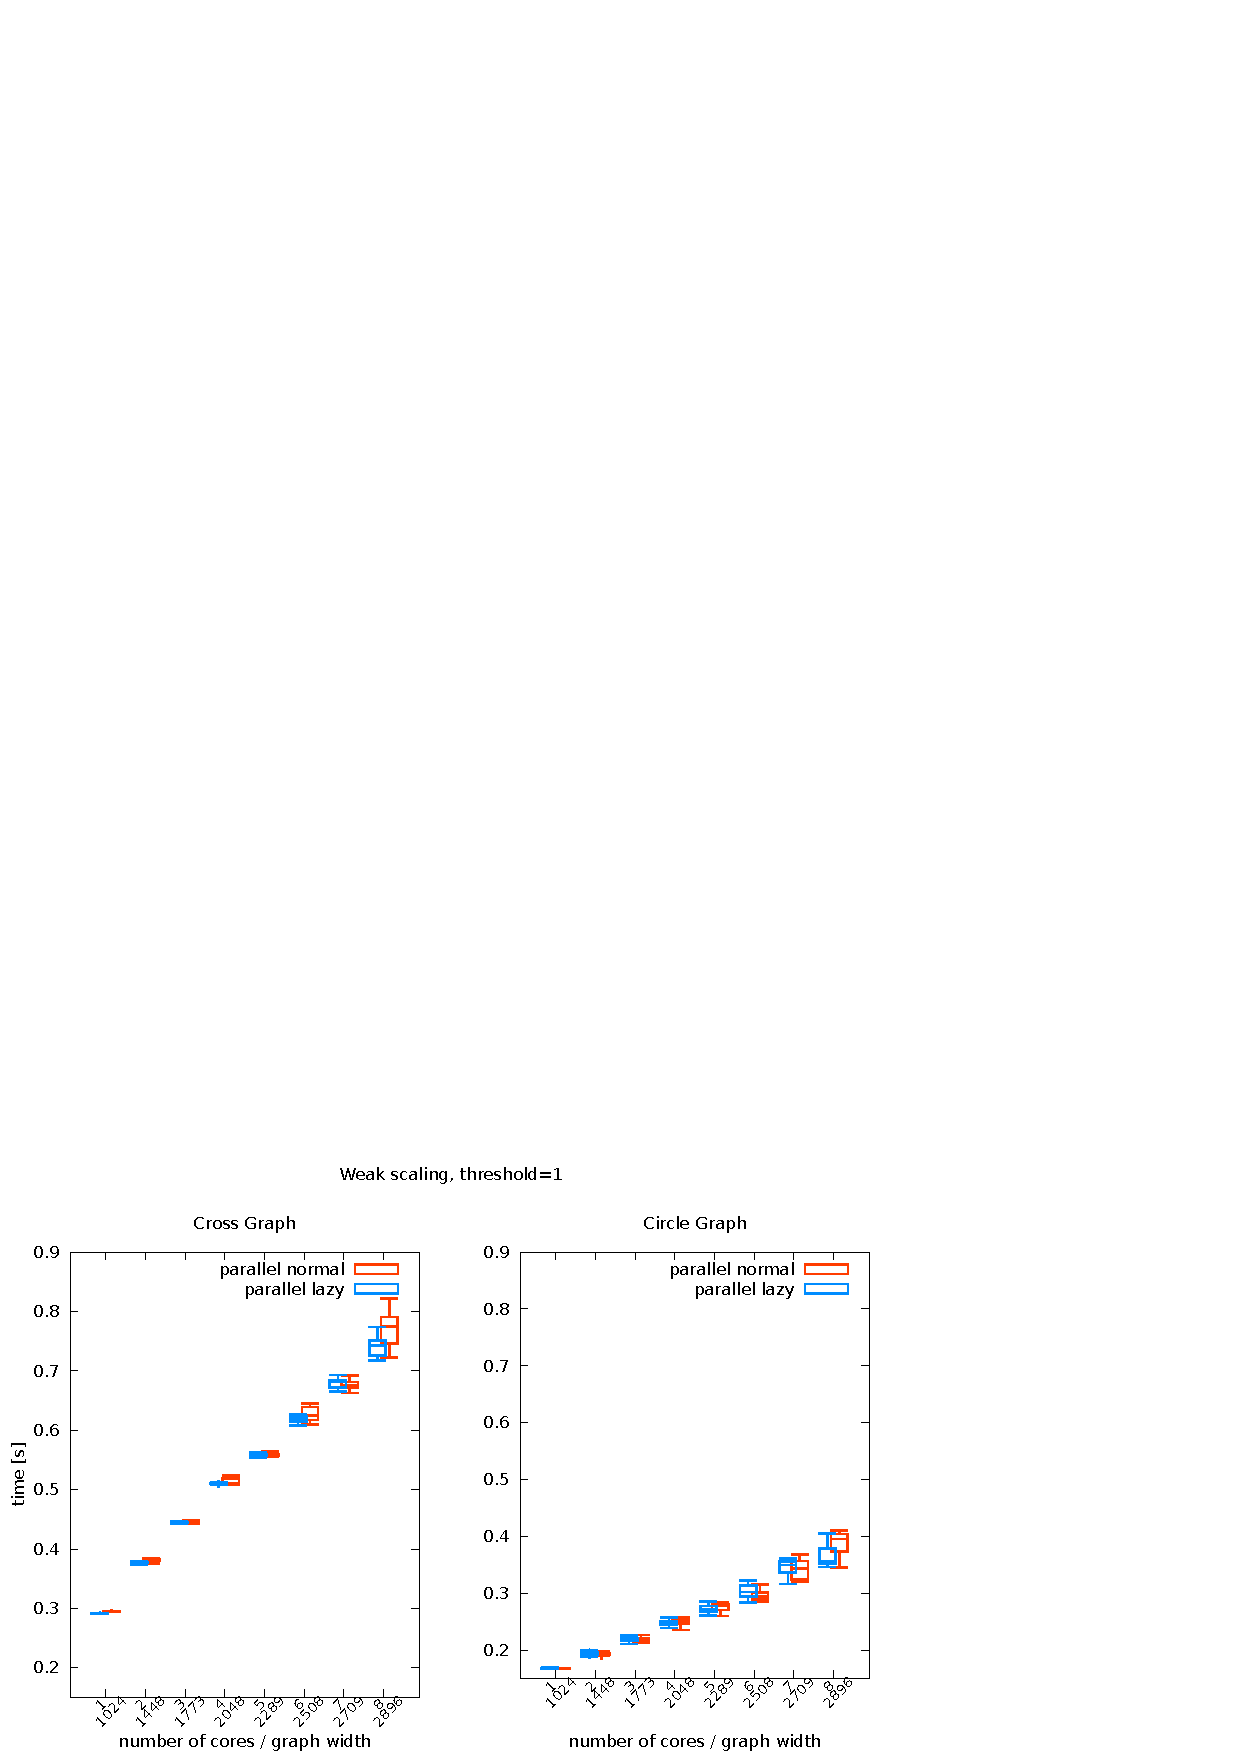
\includegraphics[height=210pt]{weak_scaling.pdf}
\end{center}
\end{frame}

%------------------------------------------------
\subsection{Path length}
\begin{frame}
\frametitle{Benchmarking: Path length $\leftrightarrow$ \# cores}
compared to A* from Boost Graph Library
\begin{center}
	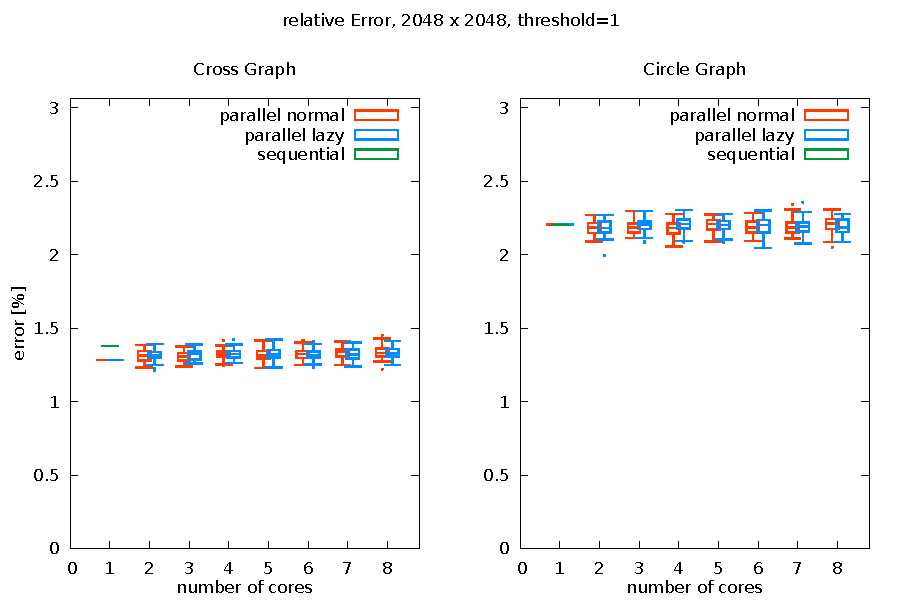
\includegraphics[height=210pt]{error_cores.pdf}
\end{center}
\end{frame}

\definecolor{0.1}{HTML}{FF3C00}
\definecolor{1}{HTML}{008CFF}
\definecolor{10}{HTML}{00993A}

\begin{frame}
\frametitle{Benchmarking: Path length $\leftrightarrow$ Threshold update}
\begin{columns}[c] % The "c" option specifies centered vertical alignment while the "t" option is used for top vertical alignment
\column{.35\textwidth} % Left column and width
\textbf{Threshold update}
\begin{itemize}
\item \textcolor{0.1}{threshold += \textbf{0.1}}
\item \textcolor{1}{threshold += \textbf{1}}
\item \textcolor{10}{threshold += \textbf{10}}
\end{itemize}

\column{.6\textwidth} % Right column and width
\begin{center}
	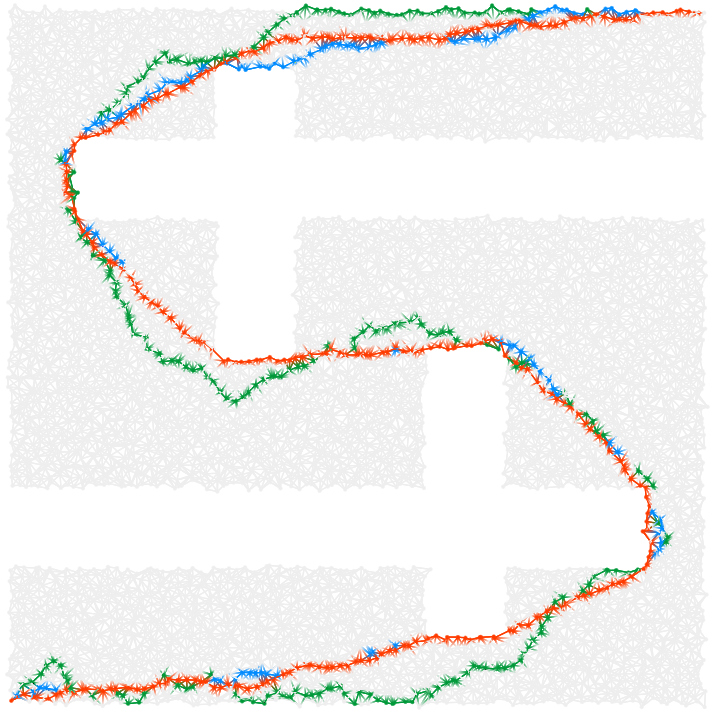
\includegraphics[height=190pt]{crossgraph.png}
\end{center}
\end{columns}
\end{frame}


\begin{frame}
\frametitle{Benchmarking: Path length $\leftrightarrow$ Threshold update}
\begin{columns}[c] % The "c" option specifies centered vertical alignment while the "t" option is used for top vertical alignment
\column{.35\textwidth} % Left column and width
\textbf{Threshold update}
\begin{itemize}
\item \textcolor{0.1}{threshold += \textbf{0.1}}
\item \textcolor{1}{threshold += \textbf{1}}
\item \textcolor{10}{threshold += \textbf{10}}
\end{itemize}

\column{.6\textwidth} % Right column and width
\begin{center}
	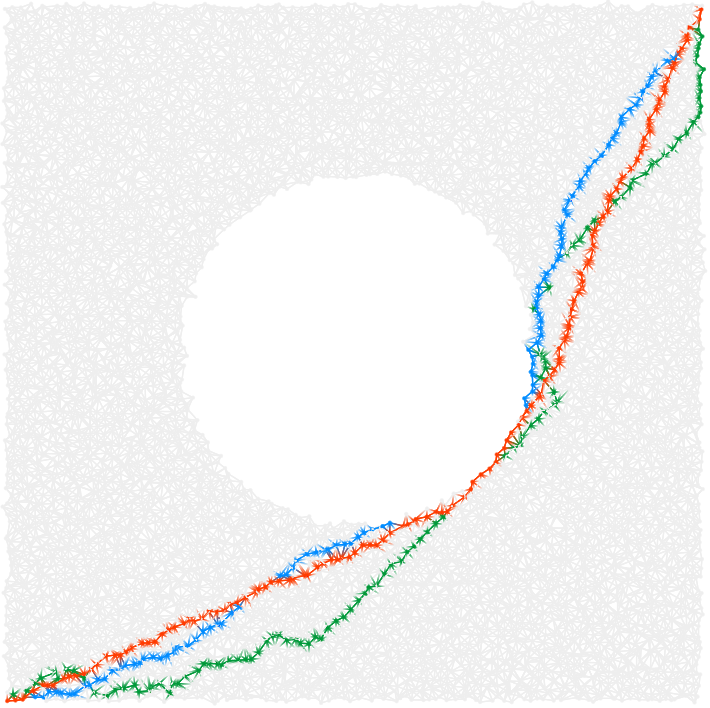
\includegraphics[height=190pt]{circlegraph.png}
\end{center}
\end{columns}
\end{frame}


\begin{frame}
\frametitle{Benchmarking: Path length $\leftrightarrow$ Threshold update}
\begin{columns}[c] % The "c" option specifies centered vertical alignment while the "t" option is used for top vertical alignment
\column{.35\textwidth} % Left column and width
\textbf{Threshold update}
\begin{itemize}
\item \textcolor{0.1}{threshold += \textbf{0.1}}
\item \textcolor{1}{threshold += \textbf{1}}
\item \textcolor{10}{threshold += \textbf{10}}
\end{itemize}

\column{.6\textwidth} % Right column and width
\begin{center}
	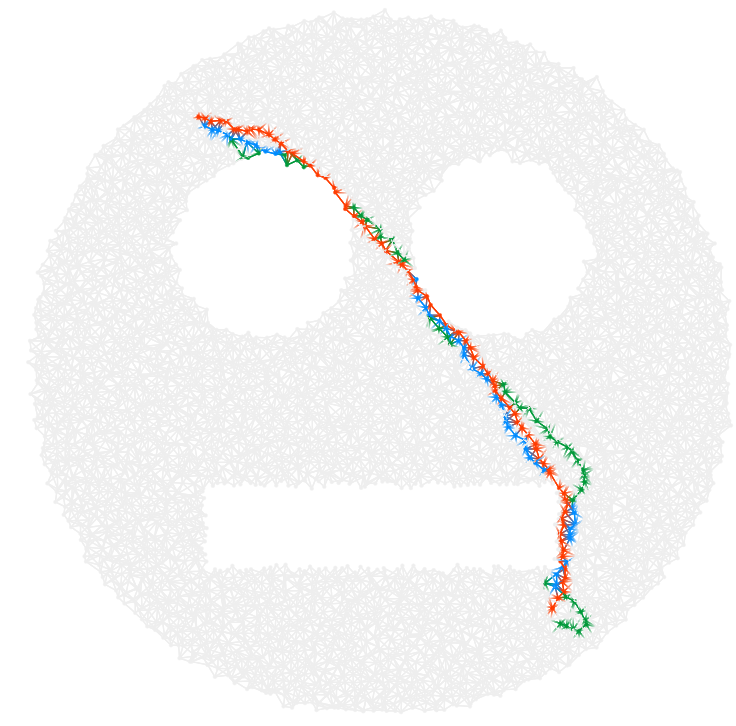
\includegraphics[height=190pt]{smileygraph.png}
\end{center}
\end{columns}
\end{frame}


\begin{frame}
\frametitle{Benchmarking: Path length $\leftrightarrow$ Threshold update}
compared to A* from Boost Graph Library
\begin{center}
	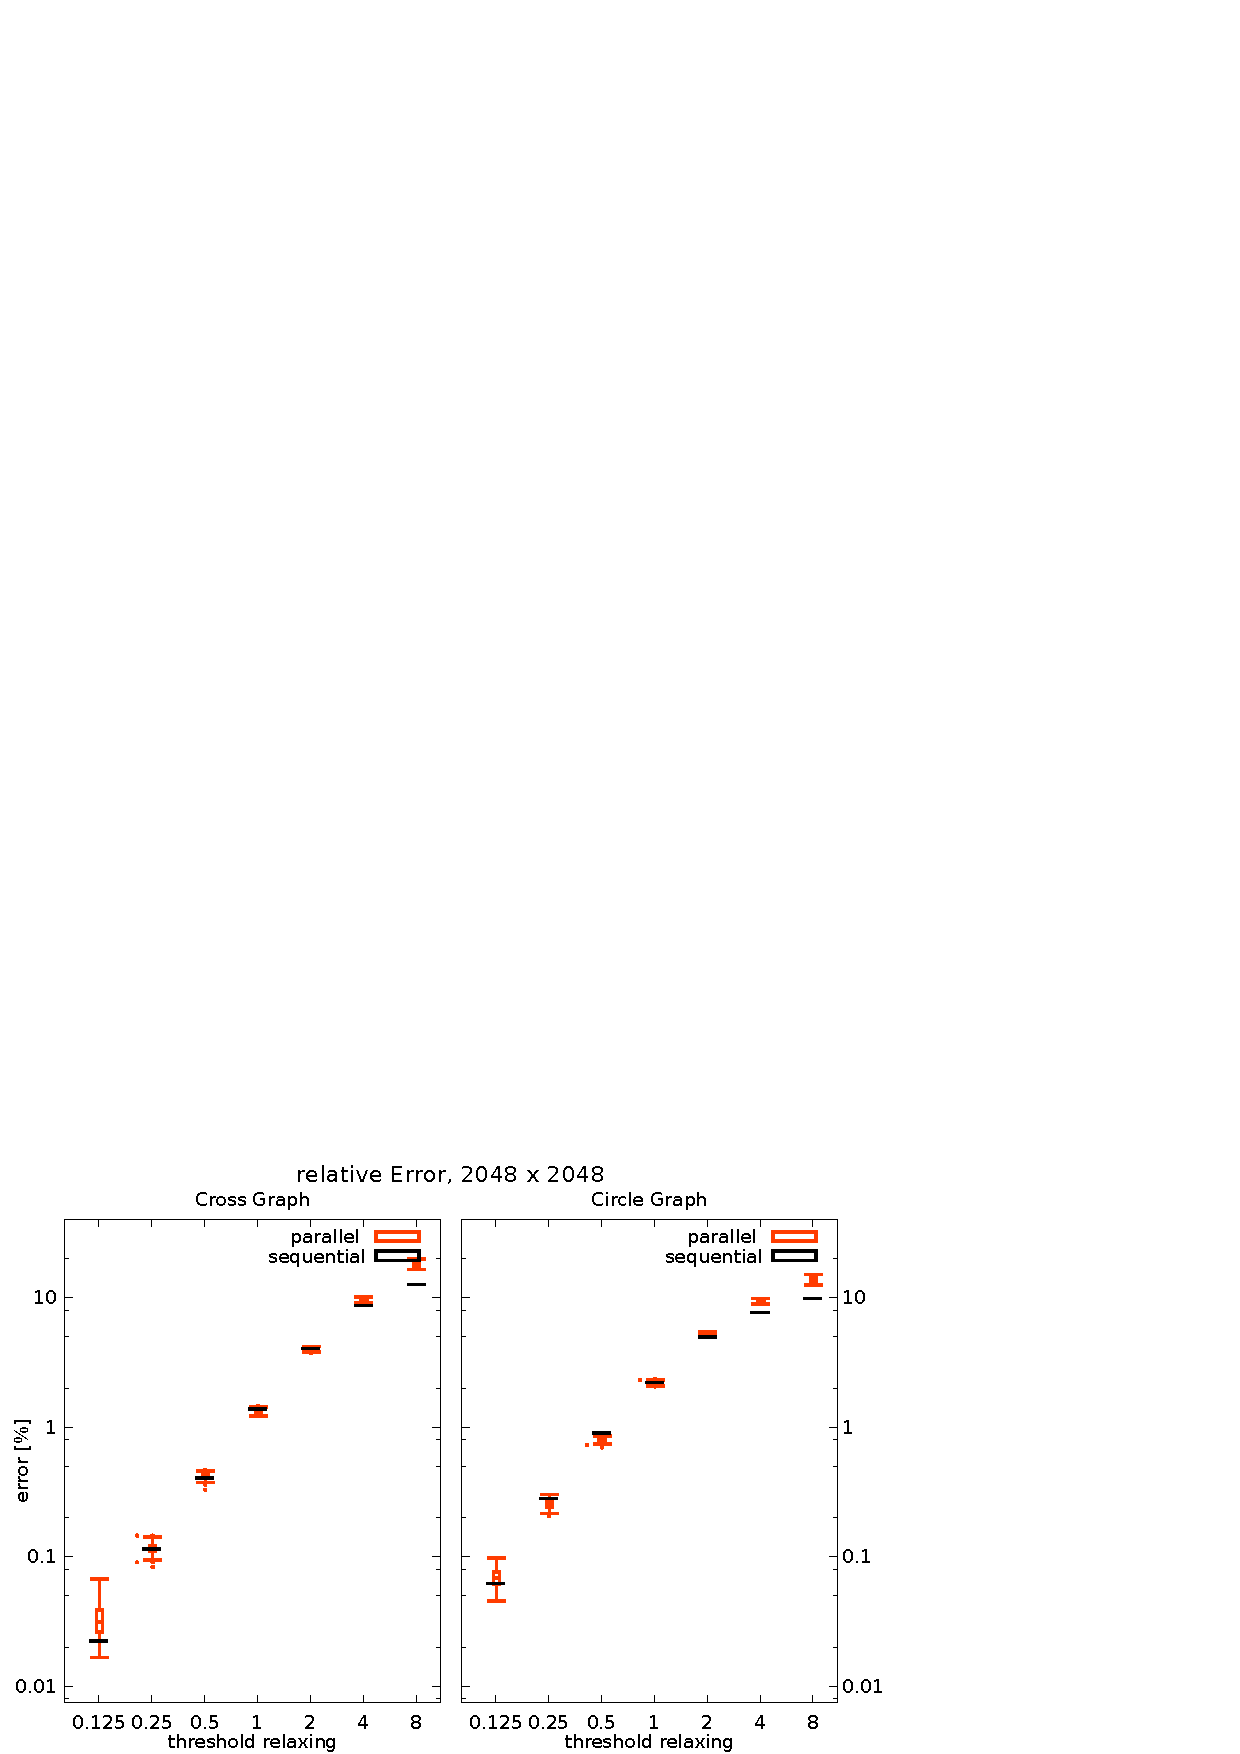
\includegraphics[height=210pt]{error_threshold.pdf}
\end{center}
\end{frame}

%------------------------------------------------
\subsection{Threshold handling}
\begin{frame}
\frametitle{Benchmarking: Run time $\leftrightarrow$ Threshold update}
\begin{center}
	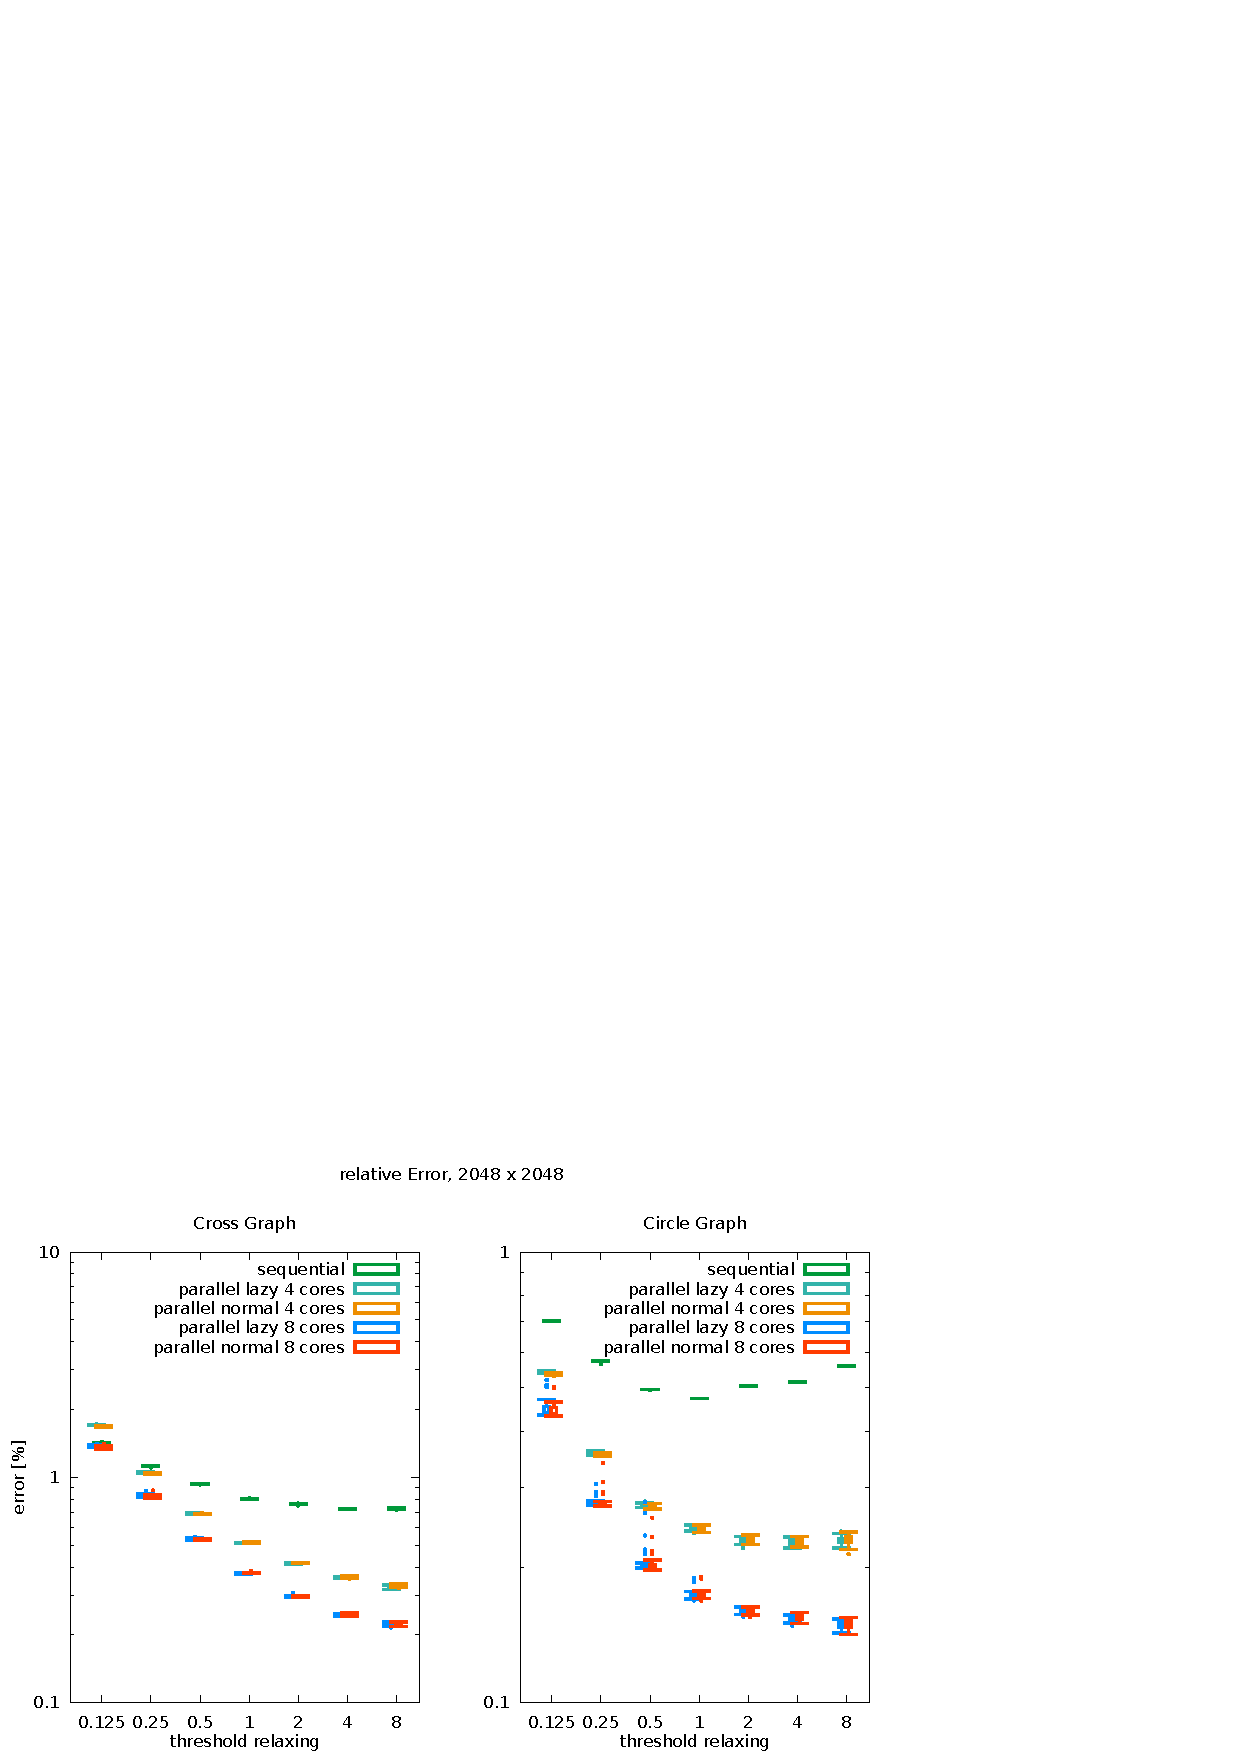
\includegraphics[height=210pt]{runtime_threshold.pdf}
\end{center}
\end{frame}

%------------------------------------------------
\section{Conclusions}
%------------------------------------------------
\begin{frame}
\frametitle{Conclusions}
In general Fringe Search is a good single source shortest path algorithm, that can be very well implemented in parallel.\\
\begin{itemize}
\item Path quality not dependent of \# cores
\item Good strong scaling
\item Weak scaling is not perfect
\item quality $\leftrightarrow$ runtime trade-off can be tuned for desired result
\end{itemize}
\end{frame}



%------------------------------------------------
\begin{frame}
\frametitle{References / Related Work}
\footnotesize{
\begin{thebibliography}{99} % Beamer does not support BibTeX so references must be inserted manually as below
\bibitem[yngvi, 2005]{p1} Yngvi Björnsson, Markus Enzenberger, Robert C. Holte and Jonathan Schaeffer (2005)
\newblock Fringe Search: Beating A* at Pathfinding on Game Maps
\newblock \emph{Proceedings of the 2005 IEEE Symposium on Computational Intelligence and Games (CIG05), Essex University, Colchester, Essex, UK, 4-6 April, 2005}
\bibitem[brand, 2009]{p1} Sandy Brand (2009)
\newblock Efficient obstacle avoidance using autonomously generated navigation meshes
\newblock \emph{Master Thesis} (Delft University of Technology)
\bibitem[brand, 2012]{p1} Sandy Brand and Rafael Bidarra (2012)
\newblock Multi-core scalable and efficient pathfinding with
Parallel Ripple Search
\newblock \emph{Computer Animation and Virtual Worlds, Volume 23, Issue 2} 2012, pp 73 -- 85.
\end{thebibliography}
}
\end{frame}


%
%\begin{frame}
%\frametitle{Benchmark runtime}
%\begin{itemize}
%\item Runtime vs. A* from Boost Graph Library
%\item Using "cross graph" and 400 - 10'000 nodes
%\item Threshold += 1
%\item 20 runs per size
%\item Intel Core 2 P9600 @ 2.53 GHZ
%\end{itemize}
%\begin{center}
%	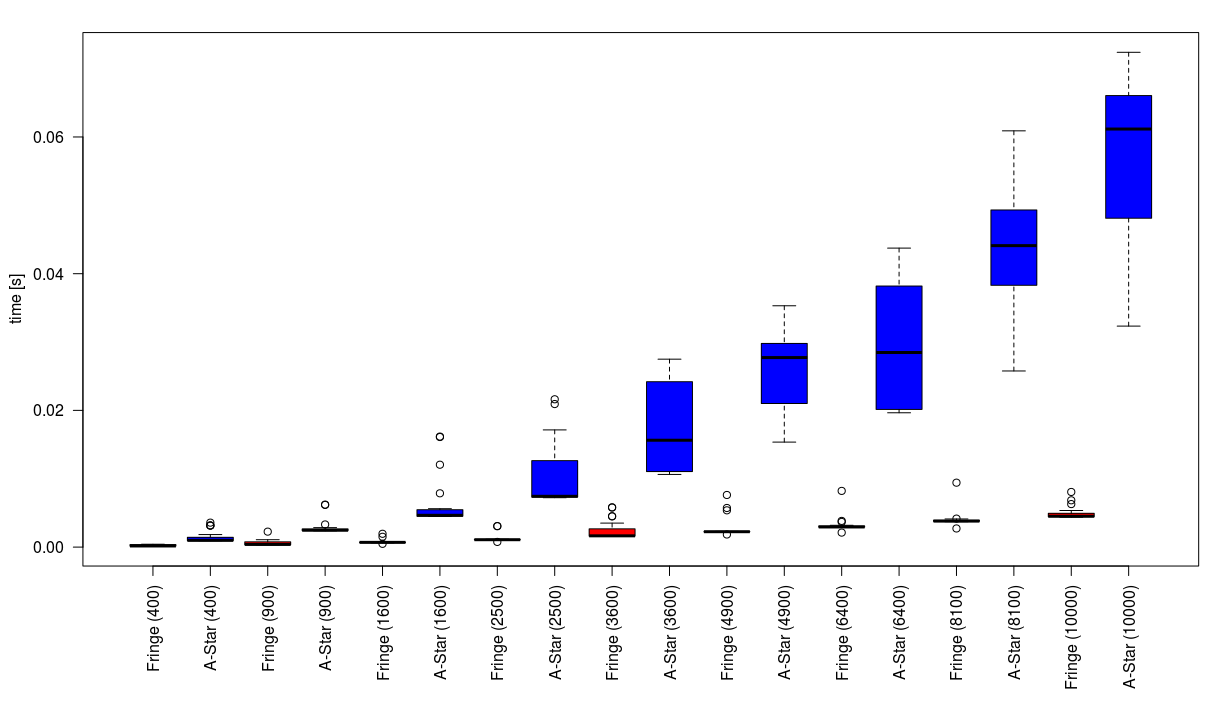
\includegraphics[height=184pt]{boxplot.png}
%\end{center}
%\end{frame}

%\begin{frame}
%\frametitle{Benchmark path length}
%\begin{itemize}
%\item Runtime vs. A* from Boost Graph Library
%\item Using "cross graph" and 400 - 10'000 nodes
%\item Threshold += 1
%\item 20 runs per size
%\item Intel Core 2 P9600 @ 2.53 GHZ
%\end{itemize}
%\end{frame}
%\begin{frame}
%\frametitle{Benchmark path length}
%\begin{center}
%    \begin{tabular}{ | r | c | c | c | c | }
%    \hline
%\# \textbf{Nodes}	&	\textbf{A-Star}	&	\textbf{Fringe}	&	\textbf{Difference} & \textbf{Difference in \%} \\ \hline
%400		&	69.731	&	70.6903	&	0.9593 & 1.37 \% \\ \hline
%900		&	101.071	&	102.638	&	1.567  & 1.55 \%\\ \hline
%1600		&	133.304	&	136.326	&	3.022 & 2.27 \% \\ \hline
%2500		&	165.47	&	167.891	&	2.421 & 1.46 \% \\ \hline
%3600		&	195.363	&	198.115	&	2.752 & 1.41 \% \\ \hline
%4900		&	227.957	&	231.554	&	3.597 & 1.58 \% \\ \hline
%6400		&	258.5	&	261.49	&	2.99  & 1.16 \% \\ \hline
%8100		&	288.961	&	293.483	&	4.522 & 1.56 \% \\ \hline
%10000	&	321.263	&	325.853	&	4.59  & 1.43 \% \\ \hline
%    \end{tabular}
%\end{center}
%
%
%\end{frame}



%\begin{frame}
%\frametitle{Project Status}
%What we still have to do:\\\quad\\
%\begin{itemize}
%\item Implement parallel version
%\item Benchmarking (strong/weak scaling)
%\item Threshold fine-tuning
%\item Write report
%\end{itemize}
%\end{frame}
%------------------------------------------------

\begin{frame}
\Huge{\centerline{The End}}
\end{frame}

%----------------------------------------------------------------------------------------

\end{document} 